%!TEX TS-program = xelatex
\documentclass[notes,12pt, aspectratio=169]{beamer}

\usepackage{amsmath,amsfonts,amssymb,amsthm,mathtools}  % пакеты для математики
\usepackage{minted}

\usepackage[english, russian]{babel} % выбор языка для документа
\usepackage[utf8]{inputenc} % задание utf8 кодировки исходного tex файла
\usepackage[X2,T2A]{fontenc}        % кодировка

\usepackage{fontspec}         % пакет для подгрузки шрифтов
\setmainfont{Helvetica}  % задаёт основной шрифт документа

% why do we need \newfontfamily:
% http://tex.stackexchange.com/questions/91507/
\newfontfamily{\cyrillicfonttt}{Helvetica}
\newfontfamily{\cyrillicfont}{Helvetica}
\newfontfamily{\cyrillicfontsf}{Helvetica}

\usepackage{unicode-math}     % пакет для установки математического шрифта
% \setmathfont{Neo Euler} % шрифт для математики

\usepackage{polyglossia}      % Пакет, который позволяет подгружать русские буквы
\setdefaultlanguage{russian}  % Основной язык документа
\setotherlanguage{english}    % Второстепенный язык документа

% Шрифт для кода
\setmonofont[Scale=0.85]{Monaco}
\usepackage{verbments}

\usepackage{pgfpages}
% These slides also contain speaker notes. You can print just the slides,
% just the notes, or both, depending on the setting below. Comment out the want
% you want.
%\setbeameroption{hide notes} % Only slide
%\setbeameroption{show only notes} % Only notes
%\setbeameroption{show notes on second screen=right} % Both

\usepackage{array}

\usepackage{tikz}
\usepackage{verbatim}
\setbeamertemplate{note page}{\pagecolor{yellow!5}\insertnote}
\usetikzlibrary{positioning}
\usetikzlibrary{snakes}
\usetikzlibrary{calc}
\usetikzlibrary{arrows}
\usetikzlibrary{decorations.markings}
\usetikzlibrary{shapes.misc}
\usetikzlibrary{matrix,shapes,arrows,fit,tikzmark}

\usepackage{hyperref}
\usepackage{lipsum}
\usepackage{multimedia}
\usepackage{multirow}
\usepackage{dcolumn}
\usepackage{bbm}
\newcolumntype{d}[0]{D{.}{.}{5}}

\usepackage{changepage}
\usepackage{appendixnumberbeamer}
\newcommand{\beginbackup}{
   \newcounter{framenumbervorappendix}
   \setcounter{framenumbervorappendix}{\value{framenumber}}
   \setbeamertemplate{footline}
   {
     \leavevmode%
     \hline
     box{%
       \begin{beamercolorbox}[wd=\paperwidth,ht=2.25ex,dp=1ex,right]{footlinecolor}%
%         \insertframenumber  \hspace*{2ex} 
       \end{beamercolorbox}}%
     \vskip0pt%
   }
 }
\newcommand{\backupend}{
   \addtocounter{framenumbervorappendix}{-\value{framenumber}}
   \addtocounter{framenumber}{\value{framenumbervorappendix}} 
}

% для имитации питоновского синтаксиса 
\newcommand{\pgr}[1]{{\color{green} \textbf{#1}}}


%%%%%%%%%% Работа с картинками %%%%%%%%%
\usepackage{graphicx}                  % Для вставки рисунков
\usepackage{graphics}
\graphicspath{{images/}}    % можно указать папки с картинками
\usepackage{wrapfig}                   % Обтекание рисунков и таблиц текстом

\usepackage[space]{grffile}
\usepackage{booktabs}

% These are my colors -- there are many like them, but these ones are mine.
\definecolor{blue}{RGB}{0,114,178}
\definecolor{red}{RGB}{213,94,0}
\definecolor{yellow}{RGB}{240,228,66}
\definecolor{green}{RGB}{0,128, 0}

\hypersetup{
  colorlinks=false,
  linkbordercolor = {white},
  linkcolor = {blue}
}


%% I use a beige off white for my background
\definecolor{MyBackground}{RGB}{255,253,218}

%% Uncomment this if you want to change the background color to something else
%\setbeamercolor{background canvas}{bg=MyBackground}

%% Change the bg color to adjust your transition slide background color!
\newenvironment{transitionframe}{
  \setbeamercolor{background canvas}{bg=yellow}
  \begin{frame}}{
    \end{frame}
}

\setbeamercolor{frametitle}{fg=blue}
\setbeamercolor{title}{fg=black}
\setbeamertemplate{footline}[frame number]
\setbeamertemplate{navigation symbols}{} 
\setbeamertemplate{itemize items}{-}
\setbeamercolor{itemize item}{fg=blue}
\setbeamercolor{itemize subitem}{fg=blue}
\setbeamercolor{enumerate item}{fg=blue}
\setbeamercolor{enumerate subitem}{fg=blue}
\setbeamercolor{button}{bg=MyBackground,fg=blue,}


% If you like road maps, rather than having clutter at the top, have a roadmap show up at the end of each section 
% (and after your introduction)
% Uncomment this is if you want the roadmap!
% \AtBeginSection[]
% {
%    \begin{frame}
%        \frametitle{Roadmap of Talk}
%        \tableofcontents[currentsection]
%    \end{frame}
% }
\setbeamercolor{section in toc}{fg=blue}
\setbeamercolor{subsection in toc}{fg=red}
\setbeamersize{text margin left=1em,text margin right=1em} 

% списки, которые растягиваются на всю величину слайда 
\newenvironment{wideitemize}{\itemize\addtolength{\itemsep}{10pt}}{\enditemize}


\title[]{\textcolor{blue}{Глубокое обучение и вообще}}
\author{Ульянкин Филипп}
\date{\today}


\begin{document}

%%% TIKZ STUFF
\tikzset{   
        every picture/.style={remember picture,baseline},
        every node/.style={anchor=base,align=center,outer sep=1.5pt},
        every path/.style={thick},
        }
\newcommand\marktopleft[1]{%
    \tikz[overlay,remember picture] 
        \node (marker-#1-a) at (-.3em,.3em) {};%
}
\newcommand\markbottomright[2]{%
    \tikz[overlay,remember picture] 
        \node (marker-#1-b) at (0em,0em) {};%
}
\tikzstyle{every picture}+=[remember picture] 
\tikzstyle{mybox} =[draw=black, very thick, rectangle, inner sep=10pt, inner ysep=20pt]
\tikzstyle{fancytitle} =[draw=black,fill=red, text=white]
%%%% END TIKZ STUFF


\begin{frame}
\maketitle
\centering \textbf{\color{blue} Посиделка 5:}  Свёрточные нейронки
\end{frame}


\begin{frame}{Image recognition}
\begin{center}
	
\includegraphics[width=.8\linewidth]{pilow.png}
\end{center}
\end{frame}


\begin{frame}{Image recognition}
\begin{center}
	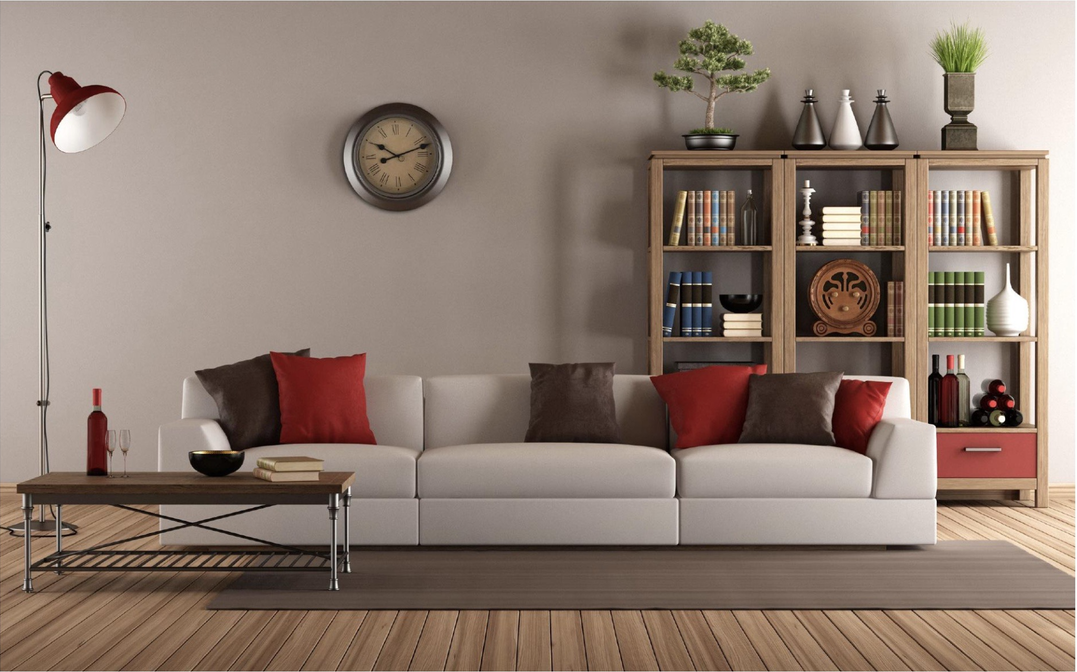
\includegraphics[width=.8\linewidth]{pilow2.png}
\end{center}
\end{frame}


\begin{frame}{Asirra captcha (2006)}
\begin{center}
	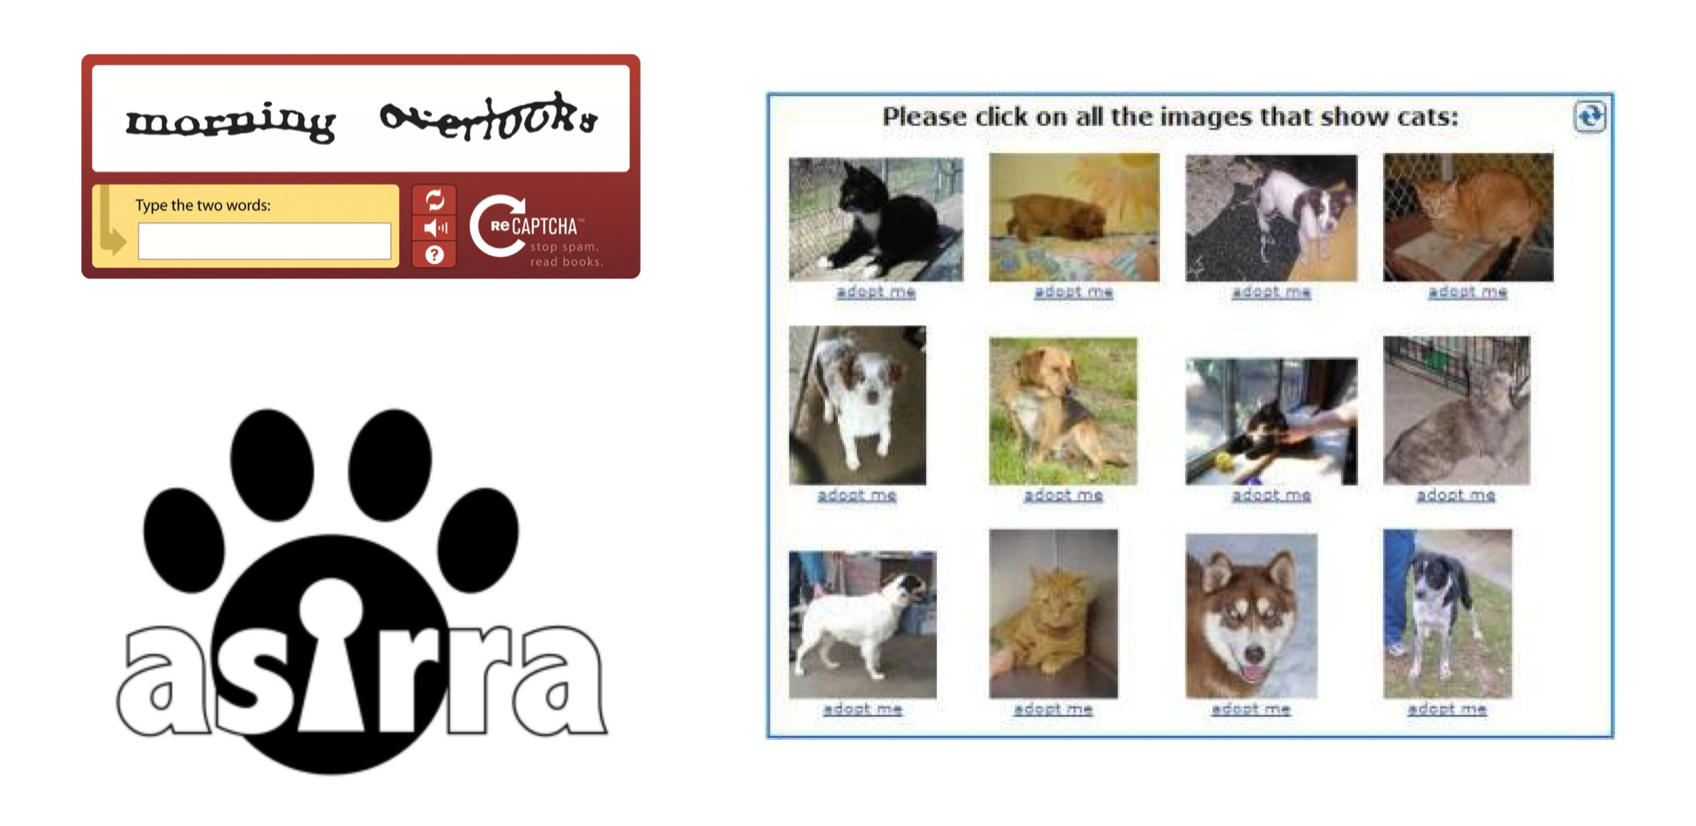
\includegraphics[width=.9\linewidth]{asira_capcha.png}
\end{center}
\end{frame}


\begin{frame}{Asirra captcha (2006)}
\begin{wideitemize}
	\item Капча портит вид сайтов, довольно бесполезная, в Microsoft придумывают в 2006 году новый вид капчи. Надо отличать котов от собак. 
	\item В то время разделение собак от кошек было очень сложной задачей, лучшая точность была $0.6$. 
	\item У нас ест 12 картинок, робот нагнёт нас с вероятностью $0.6^{12}$. 
	\item Пул картинок пополнялся фотографиями из приютов. 
\end{wideitemize} 
\end{frame}


\begin{frame}{В 2014 проект закрыли}
\begin{center}
	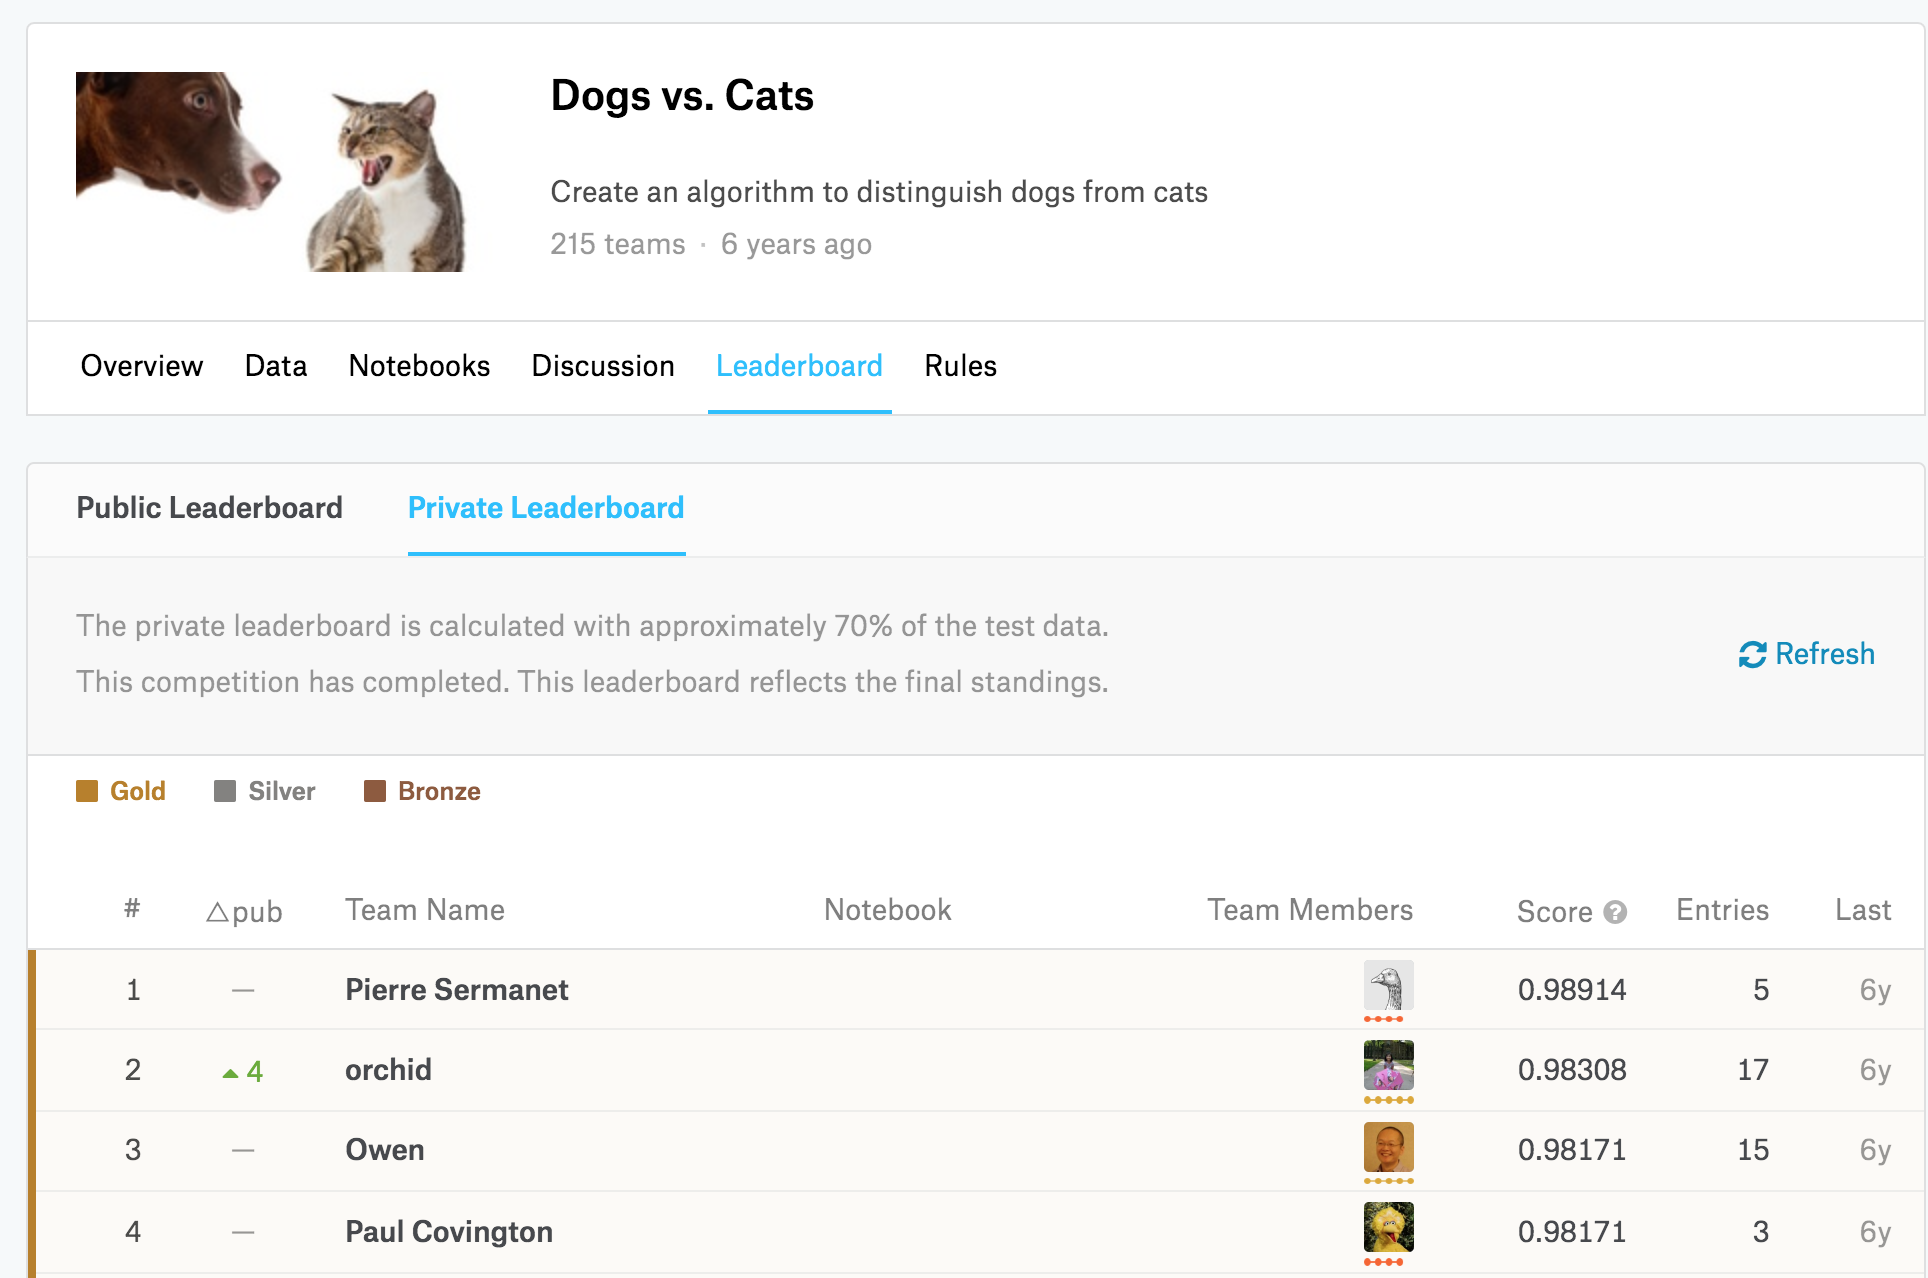
\includegraphics[width=.75\linewidth]{dogs_vs_cat.png}
\end{center}
\end{frame}



\begin{frame}{Agenda}
\begin{wideitemize}
	\item Как видит компьютер
	\item Свёртка
	\item Свёрточный слой
	\item Типичная свёрточная архитектура
	\item Что видит свёрточная нейросеть
\end{wideitemize} 
\end{frame}


\begin{transitionframe}
	\begin{center}
		\Huge Как видит компьютер
	\end{center}
\centering 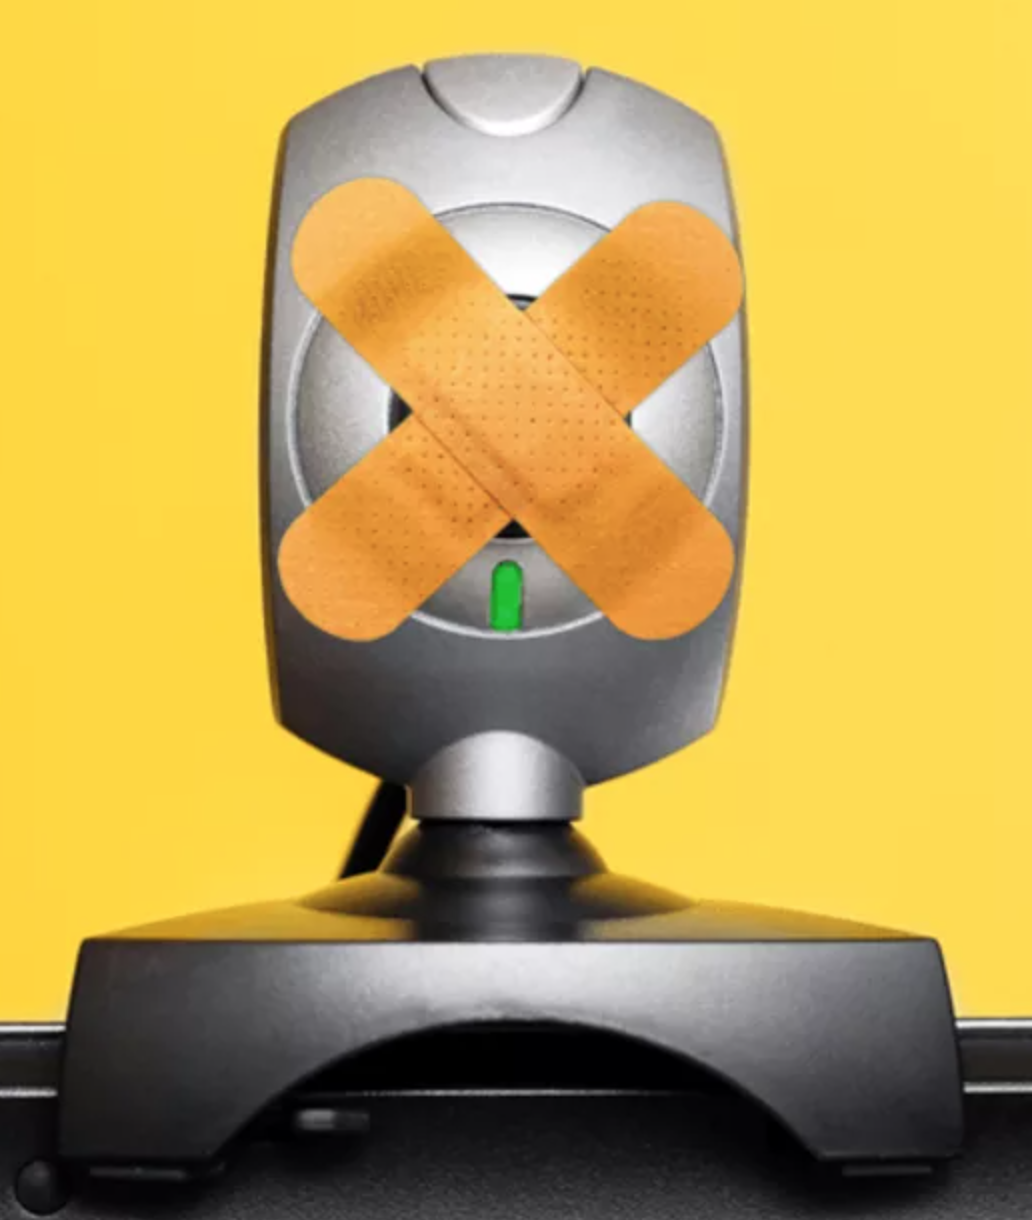
\includegraphics[scale = 0.07]{webcam.png}
\end{transitionframe}


\begin{frame}{Картинка — тензор}
\begin{itemize}
	\item Каждая картинка — это матрица из пикселей
	
	\item Каждый пиксель обладает яркостью по шкале от $0$ до $255$ 
	
\end{itemize}
\begin{center}
	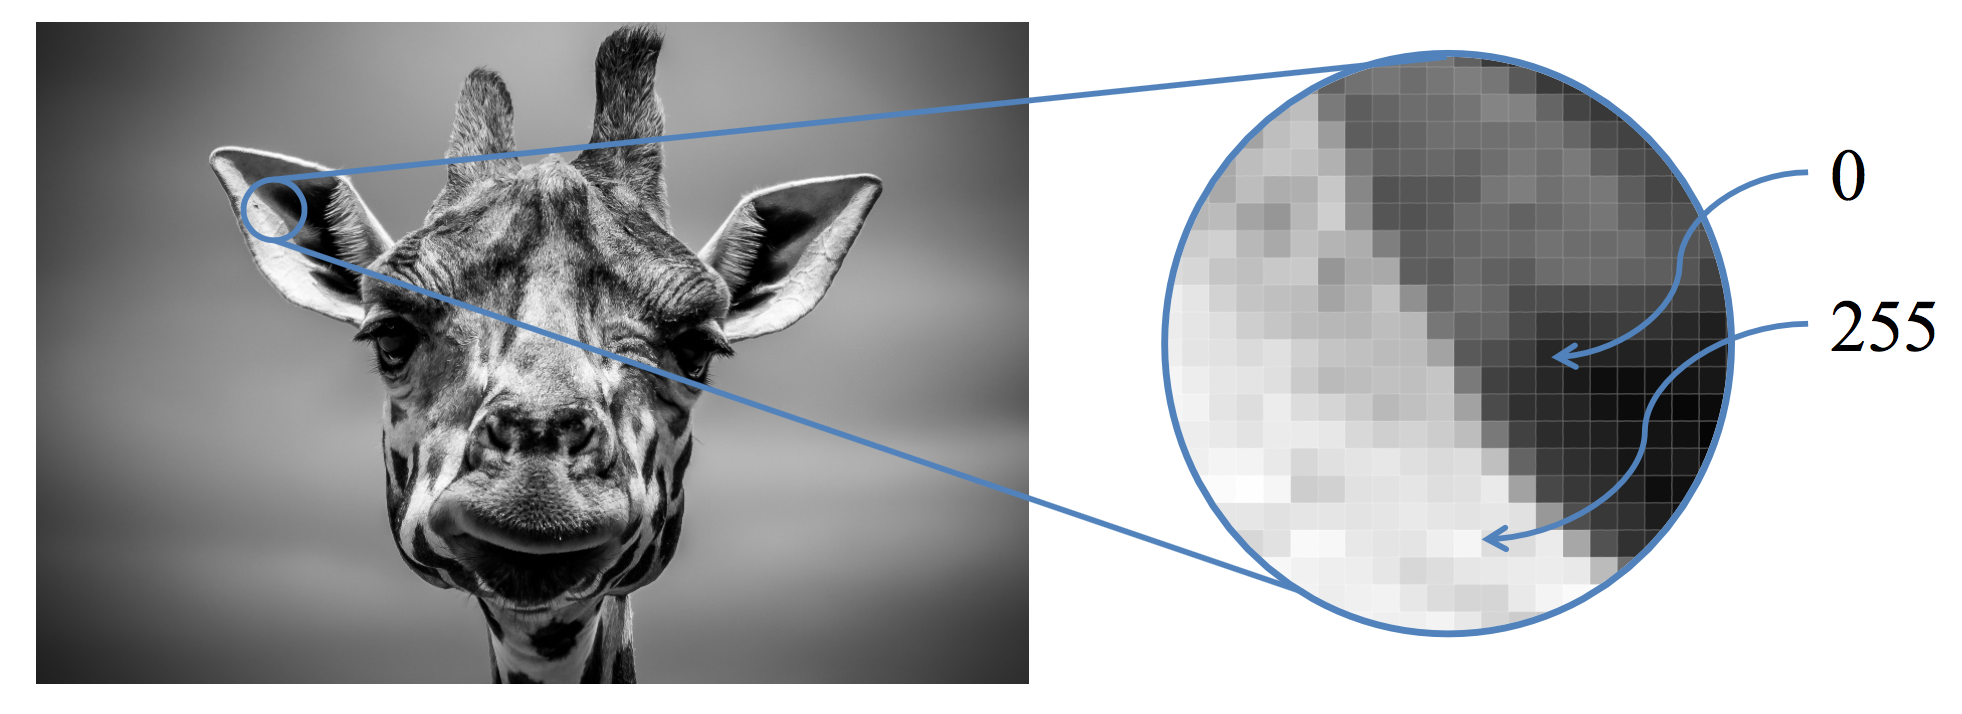
\includegraphics[width=.8\linewidth]{pixels.png}
\end{center}

\vfill %
\footnotesize
Многие слайды я нагло украл у Андрея Зимовнова: {\color{blue} \url{ https://github.com/ZEMUSHKA/mml-minor}}
\end{frame}

\begin{frame}{Картинка — тензор}
\begin{itemize}
	\item Цветное изображение имеет три канала яркости: красный, зелёный и синий (rgb)
\end{itemize}

\begin{center}
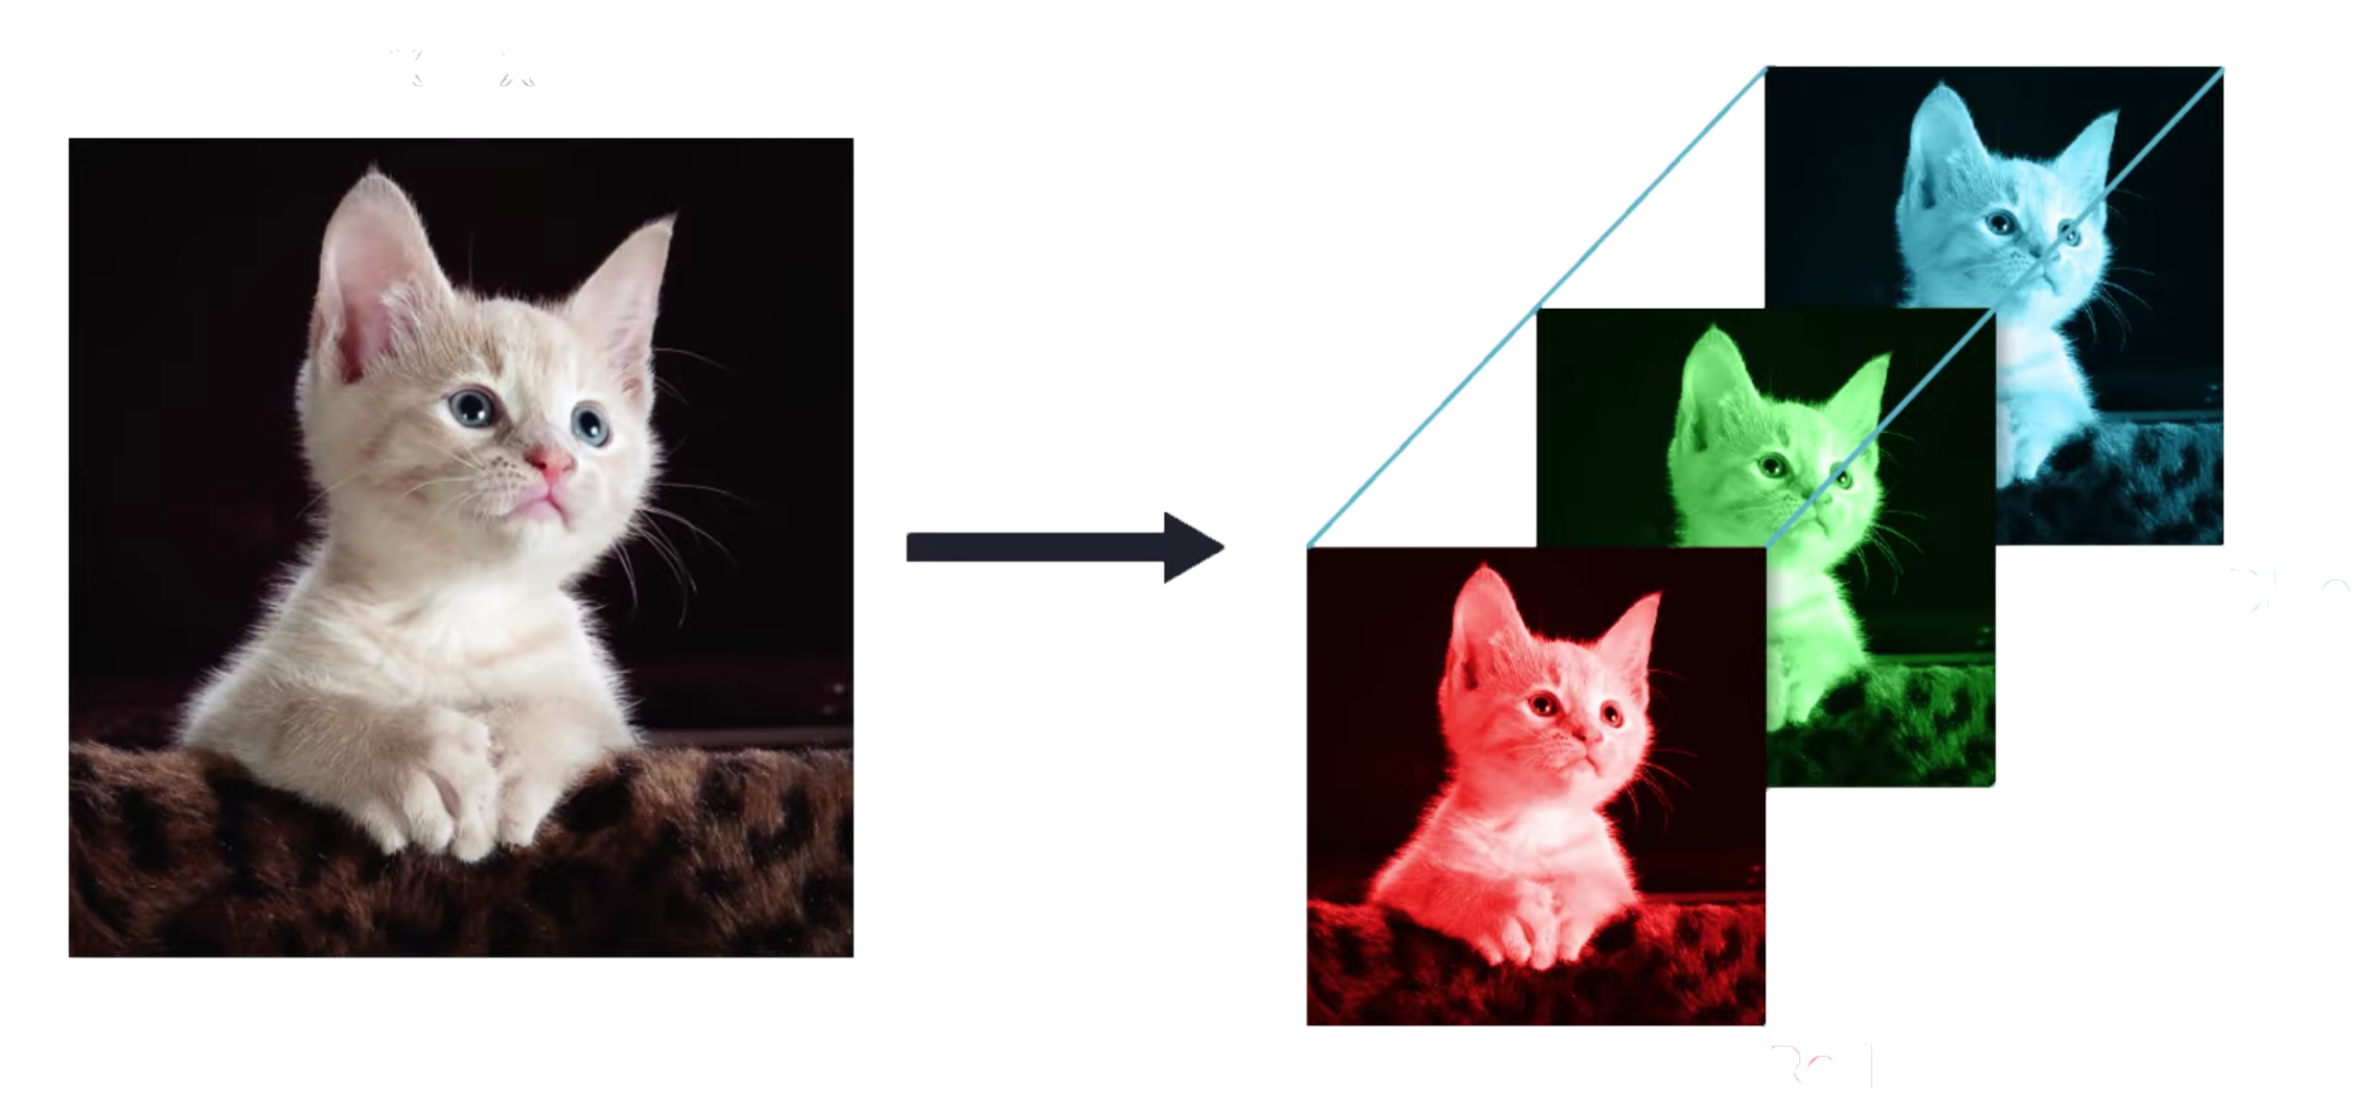
\includegraphics[width=.7\linewidth]{pixels2_clean.png}
\end{center}
\end{frame}

\begin{frame}{Картинка — тензор}
\begin{center}
	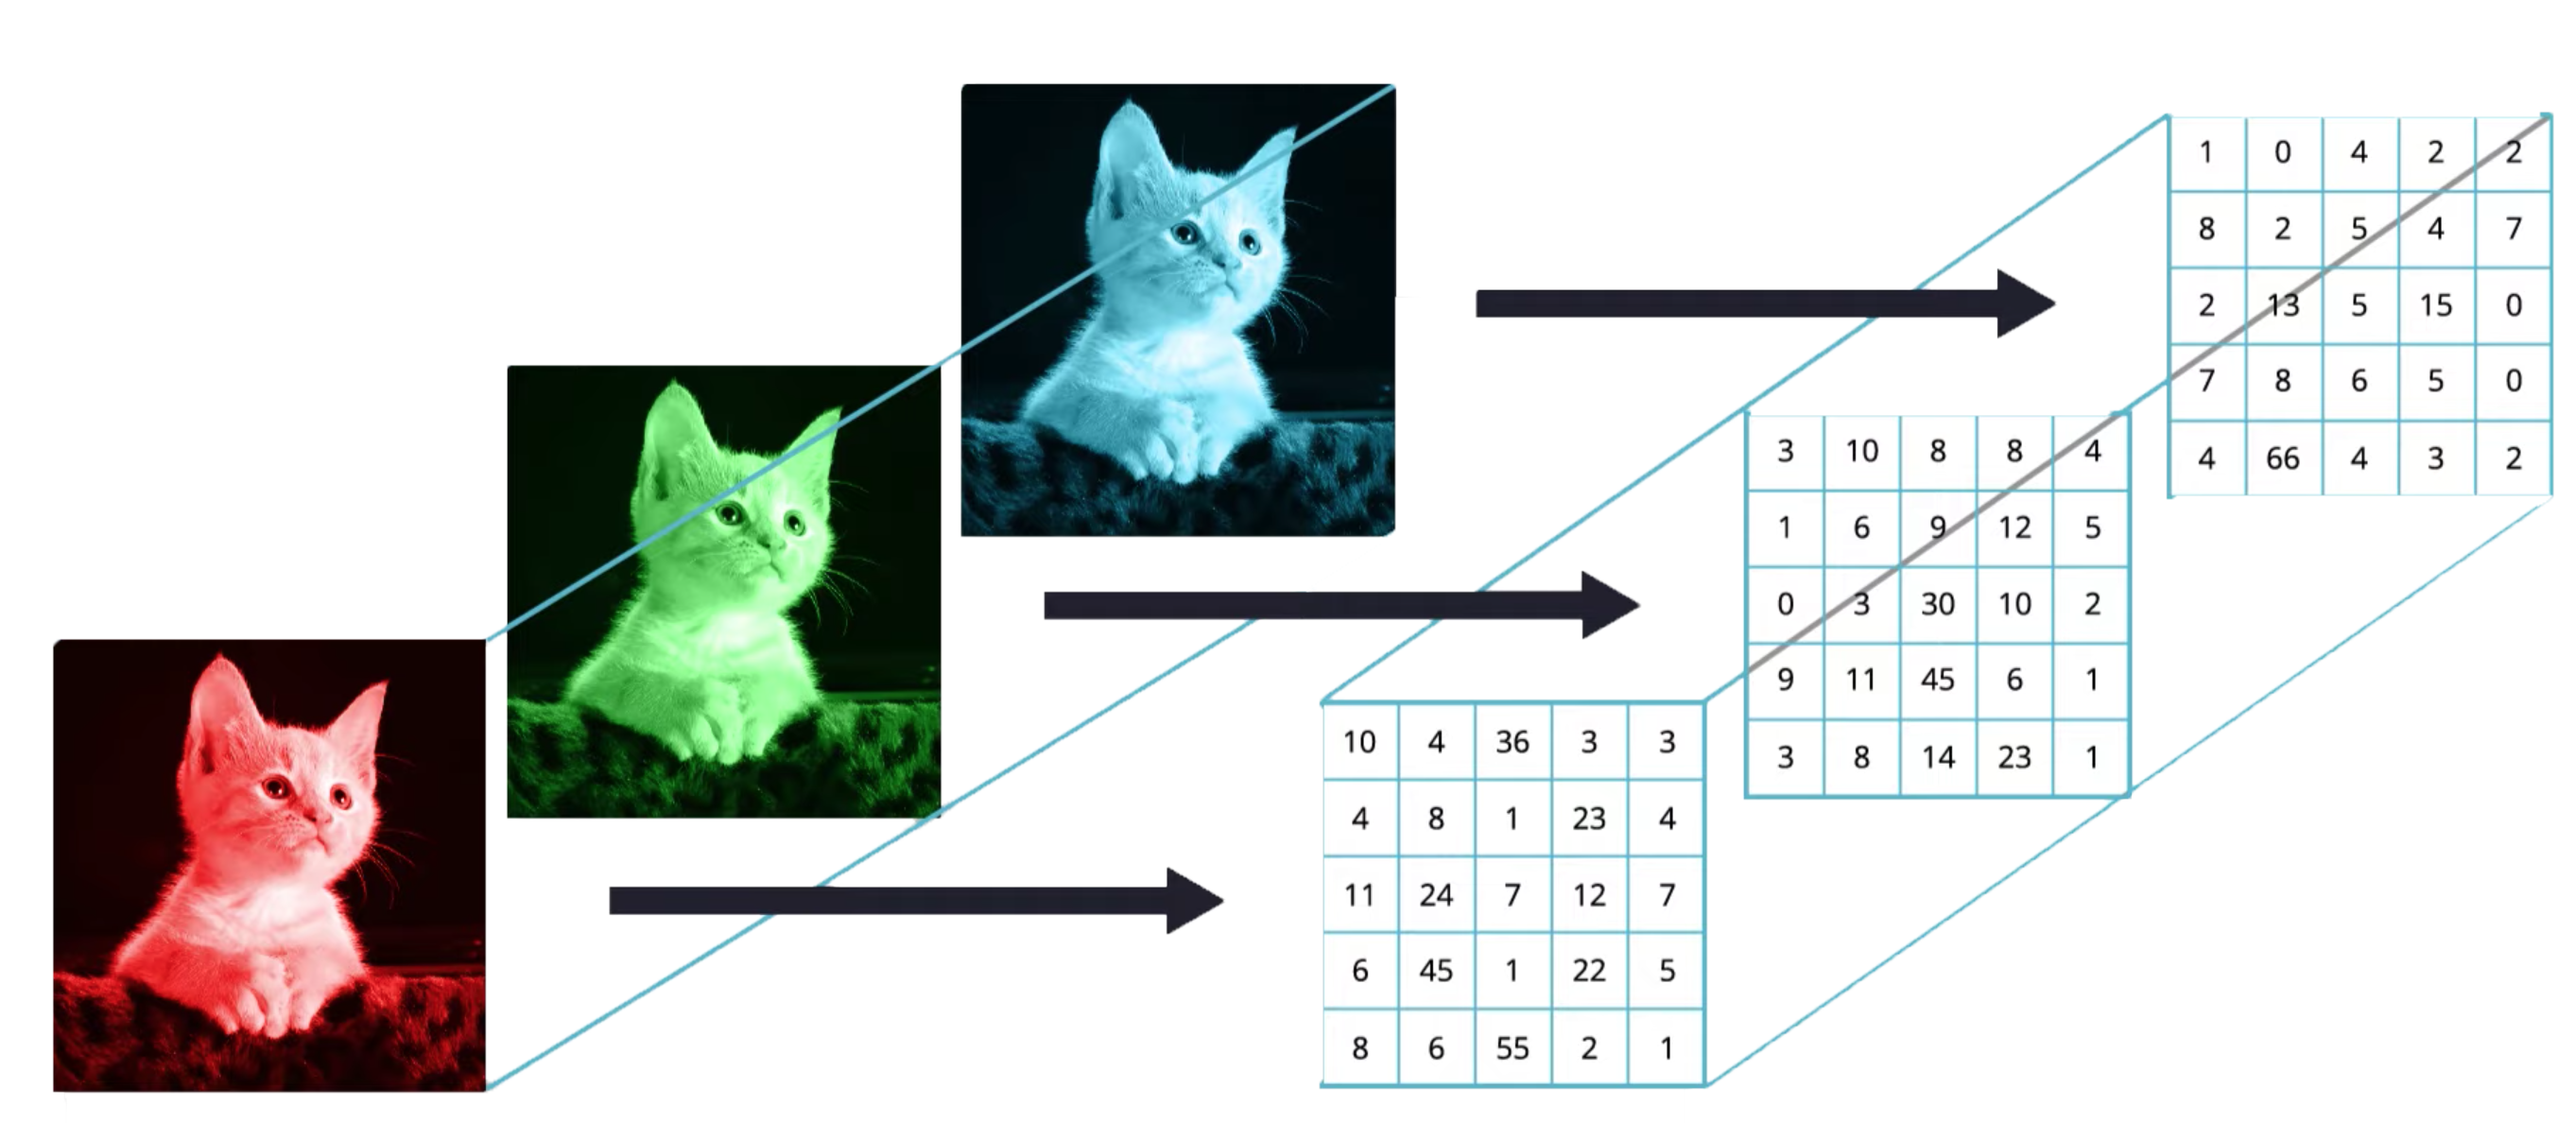
\includegraphics[width=.8\linewidth]{pixels3_clean.png}
\end{center}
\end{frame}


\begin{frame}{Картинка — тензор}
\begin{center}
	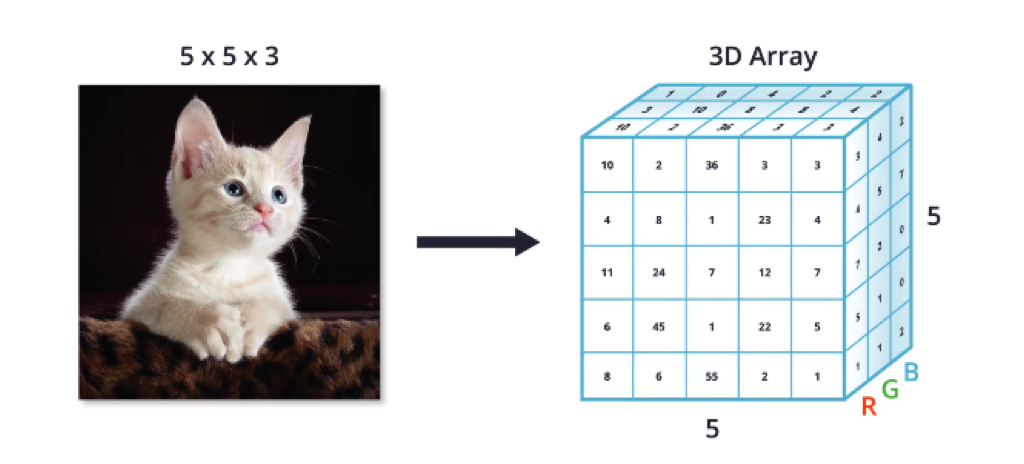
\includegraphics[width=.8\linewidth]{cat_cube.png}
\end{center}
\end{frame}


\begin{frame}{Обычная сетка}
\begin{center}
	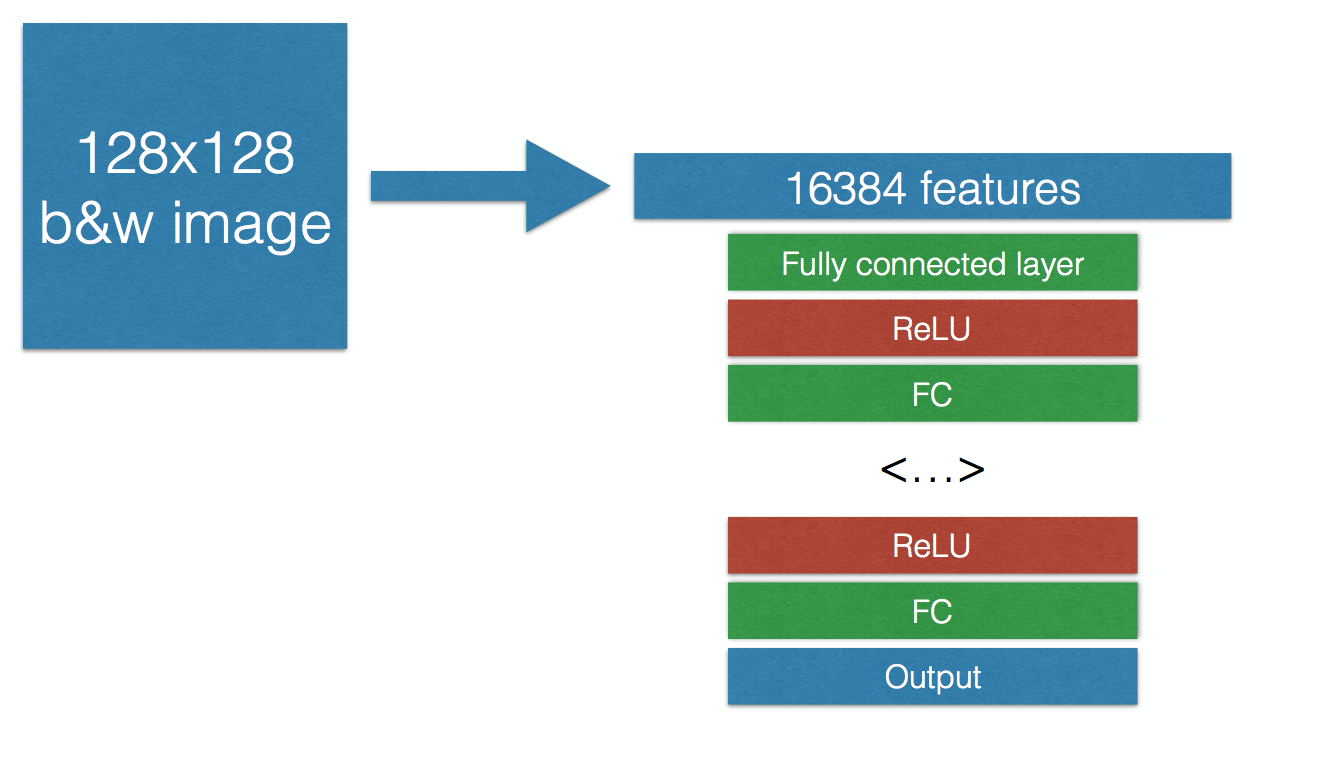
\includegraphics[width=.55\linewidth]{not_conv.png}
\end{center}

\begin{wideitemize}
	\item Развернём картинку в вектор $\Rightarrow$  \alert{очень много весов} 
	\item Если изображение немного сдвинуть, то нейрон уже не будет на него реагировать
\end{wideitemize}
\end{frame}


\begin{frame}
\begin{center}
	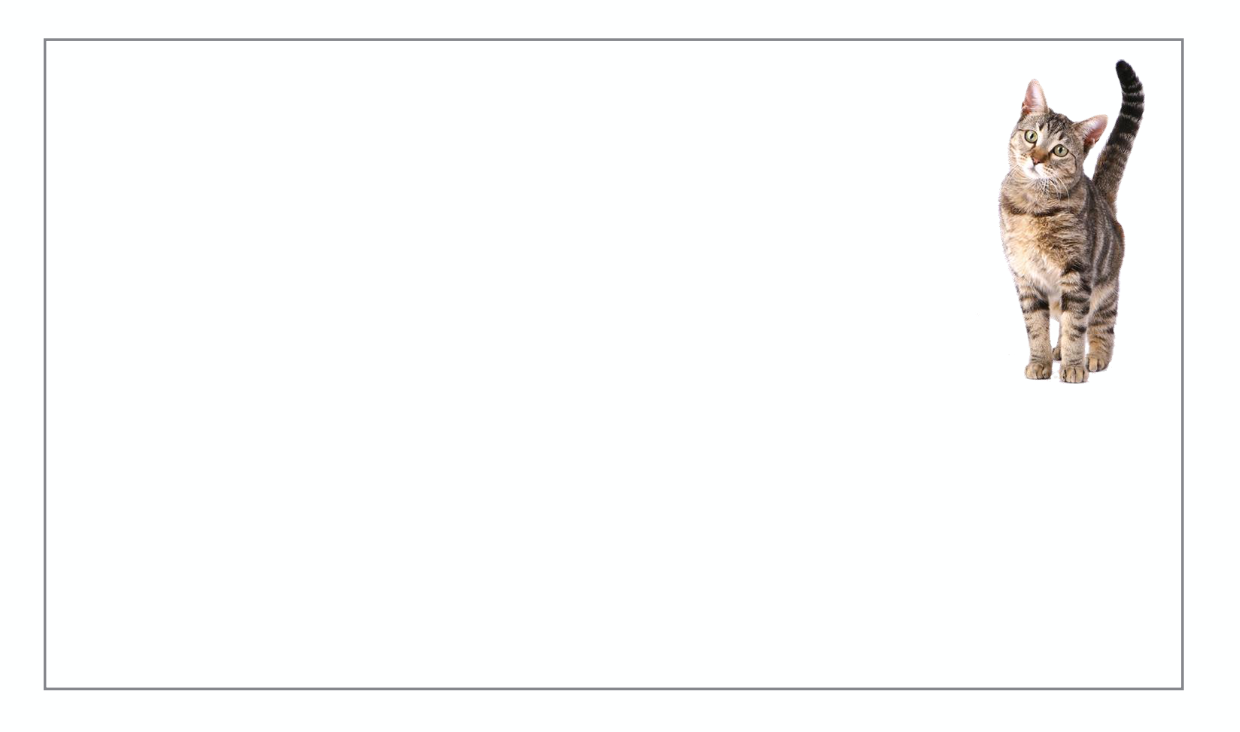
\includegraphics[width=.7\linewidth]{cat_1.png}
\end{center}
\end{frame}


\begin{frame}
\begin{center}
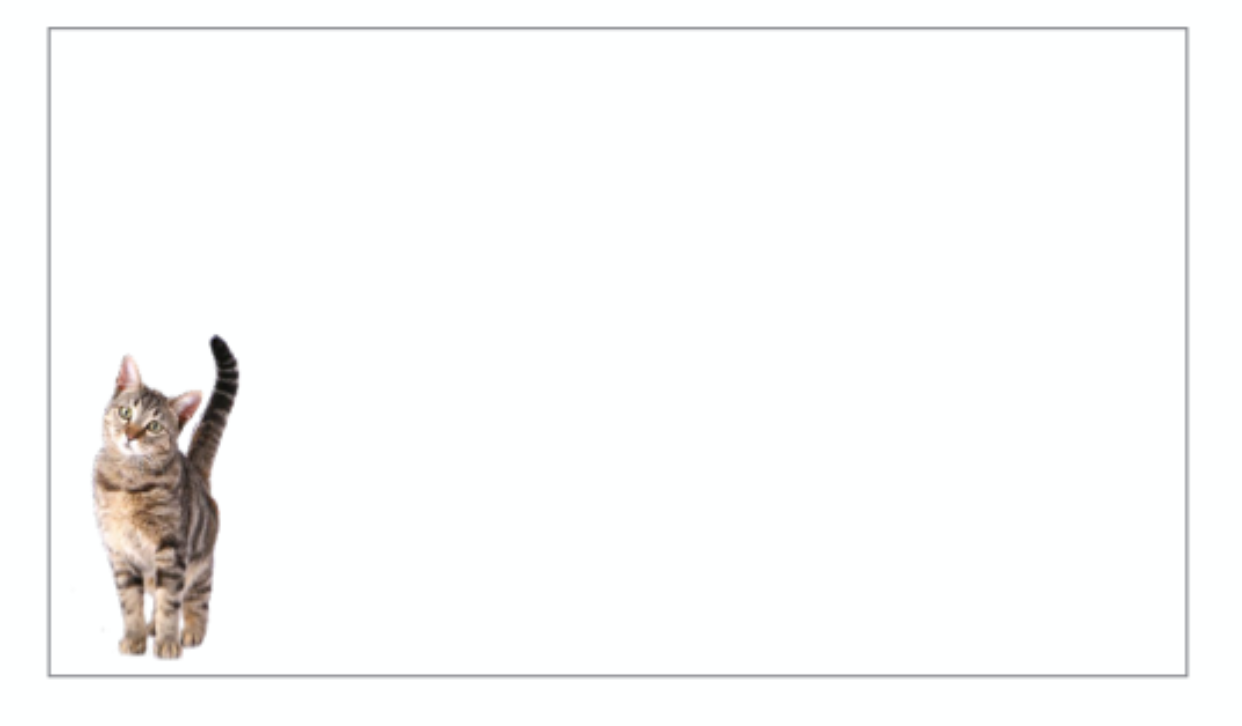
\includegraphics[width=.7\linewidth]{cat_2.png}
\end{center}
\end{frame}


\begin{frame}{Полносвязные слои для изображений}
\begin{wideitemize}
	\item  Очень много параметров
	\item  Легко могут переобучиться
	\item  Не учитывают специфику изображений (сдвиги, небольшие изменения формы и т.д.)
	\item Изображение в разных местах картинки даёт разные веса
	\item Теряется информация о взаимном расположении пикселей	
\end{wideitemize}
\end{frame}


\begin{frame}{Мы хотим, чтобы...}
\begin{wideitemize}
	\item Хотим меньше параметров, избежать переобучения
	\item Хотим, чтобы информация не терялась
	\item Хотим, чтобы модель была нечувствительна к сдвигам картинки в новые места
\end{wideitemize}

\begin{center}
	{\LARGE  \color{red} $\Rightarrow$   свёртка} 
\end{center}
\end{frame}


\begin{transitionframe}
	\begin{center}
		\Huge Свёртка
	\end{center}
\centering 
\includegraphics[scale = 0.12]{conv_tom.jpg}
\end{transitionframe}


\begin{frame}{Свёртка}
\begin{center}
	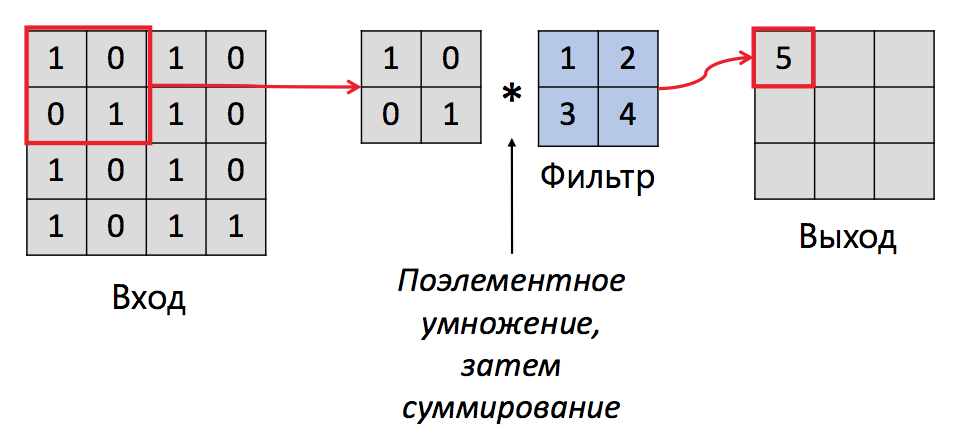
\includegraphics[width=.8\linewidth]{cconv_1.png}
\end{center}
\end{frame}

\begin{frame}{Свёртка}
\begin{center}
	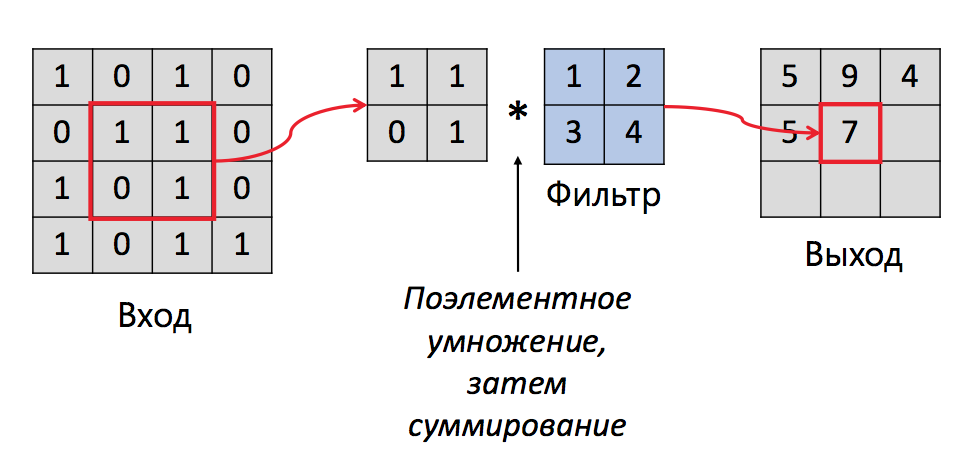
\includegraphics[width=.8\linewidth]{cconv_2.png}
\end{center}
\end{frame}


{
	\usebackgroundtemplate{ 
		% 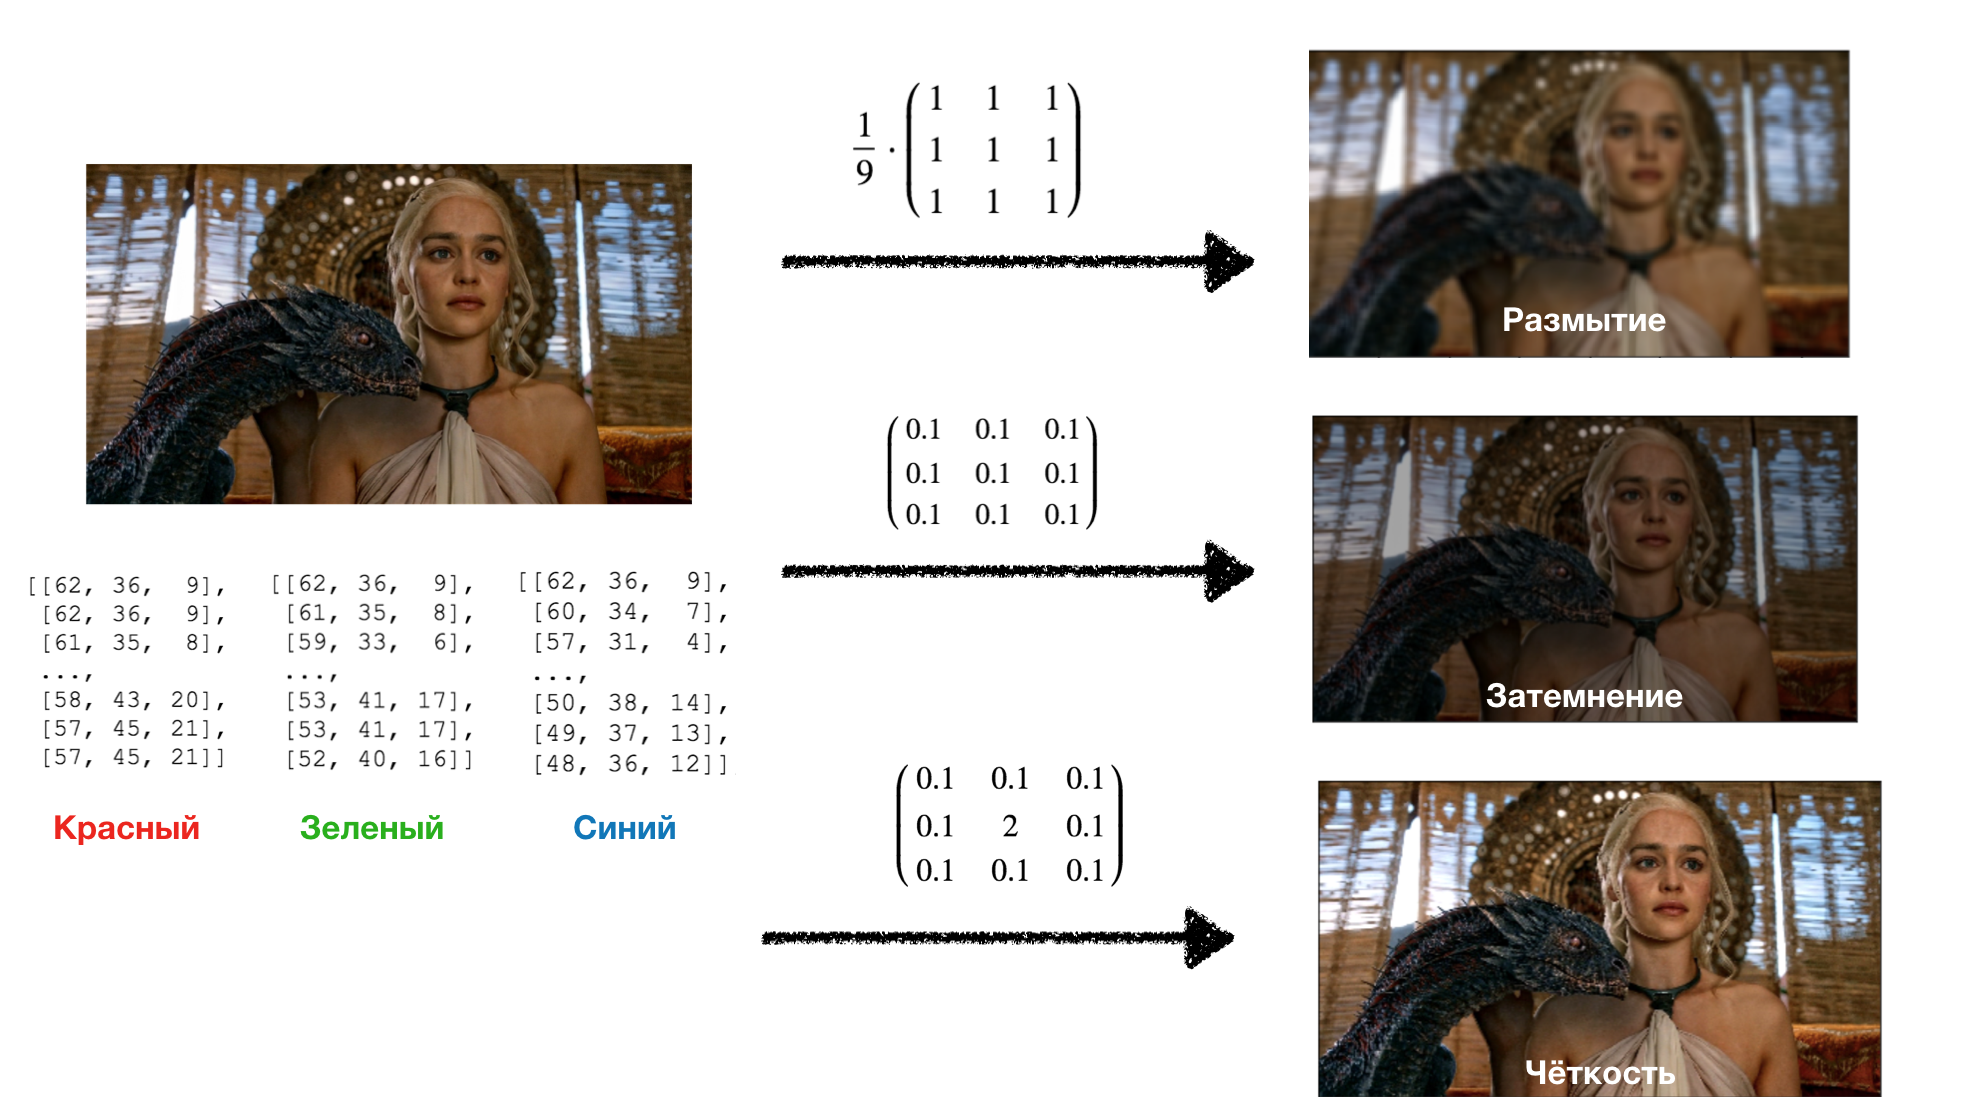
\includegraphics[width=\paperwidth]{emilia.png}}
		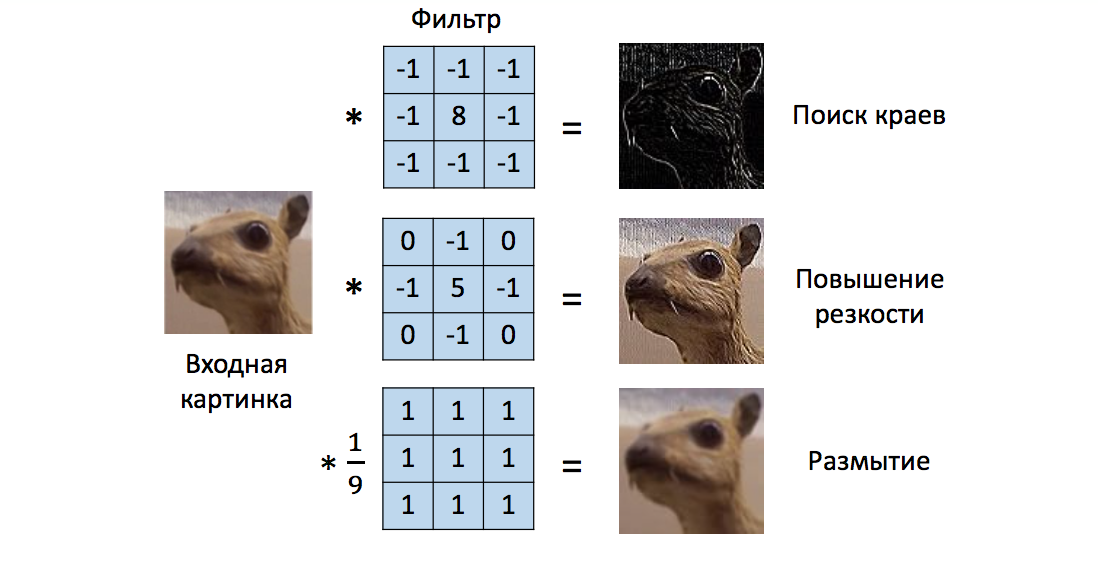
\includegraphics[width=\paperwidth]{conv_ex.png}}
	\begin{frame}
\end{frame}
}

\begin{frame}{Выделение границ} 
\[ 
\begin{pmatrix}
-1 & -1 & -1  \\
0 & 0 & 0 \\         
1 & 1 & 1 
\end{pmatrix}  \qquad 
\begin{pmatrix}
-1 & 0 & 1  \\
-1 & 0 & 1 \\         
-1 & 0 & 1 
\end{pmatrix} 
\]

\begin{center}
	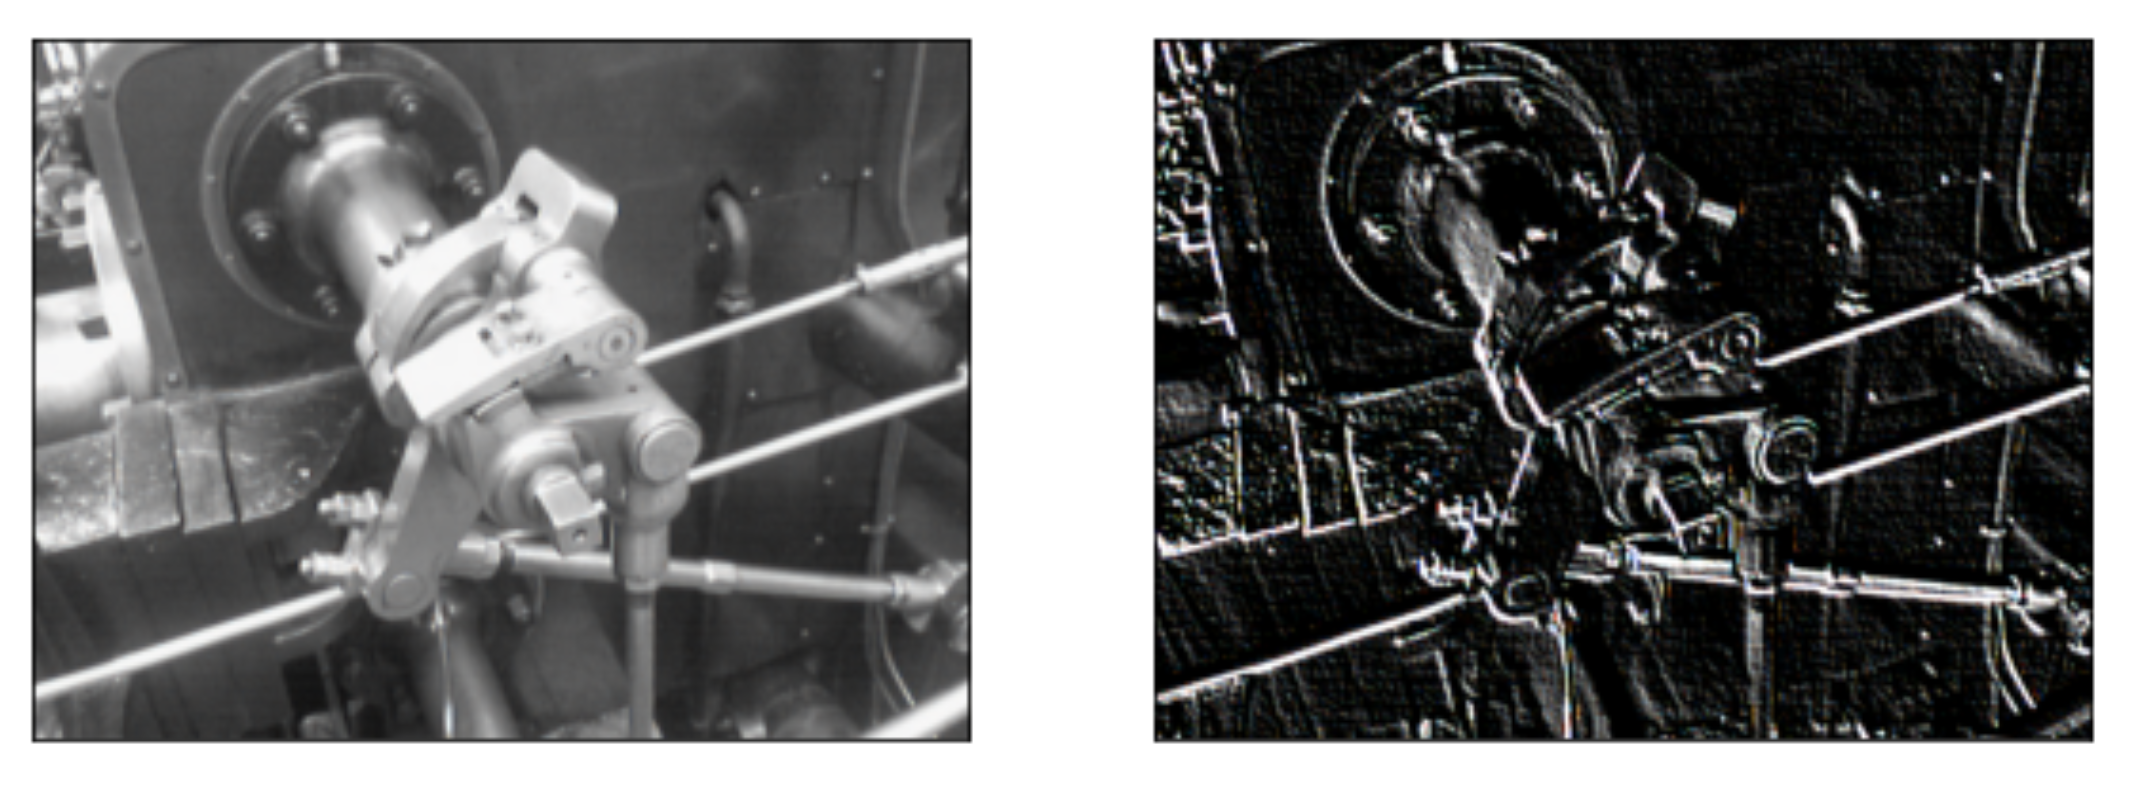
\includegraphics[width=.7\linewidth]{cconv_3.png}
\end{center}
\end{frame}


\begin{frame}{Можно комбинировать ядра} 
\begin{center}
	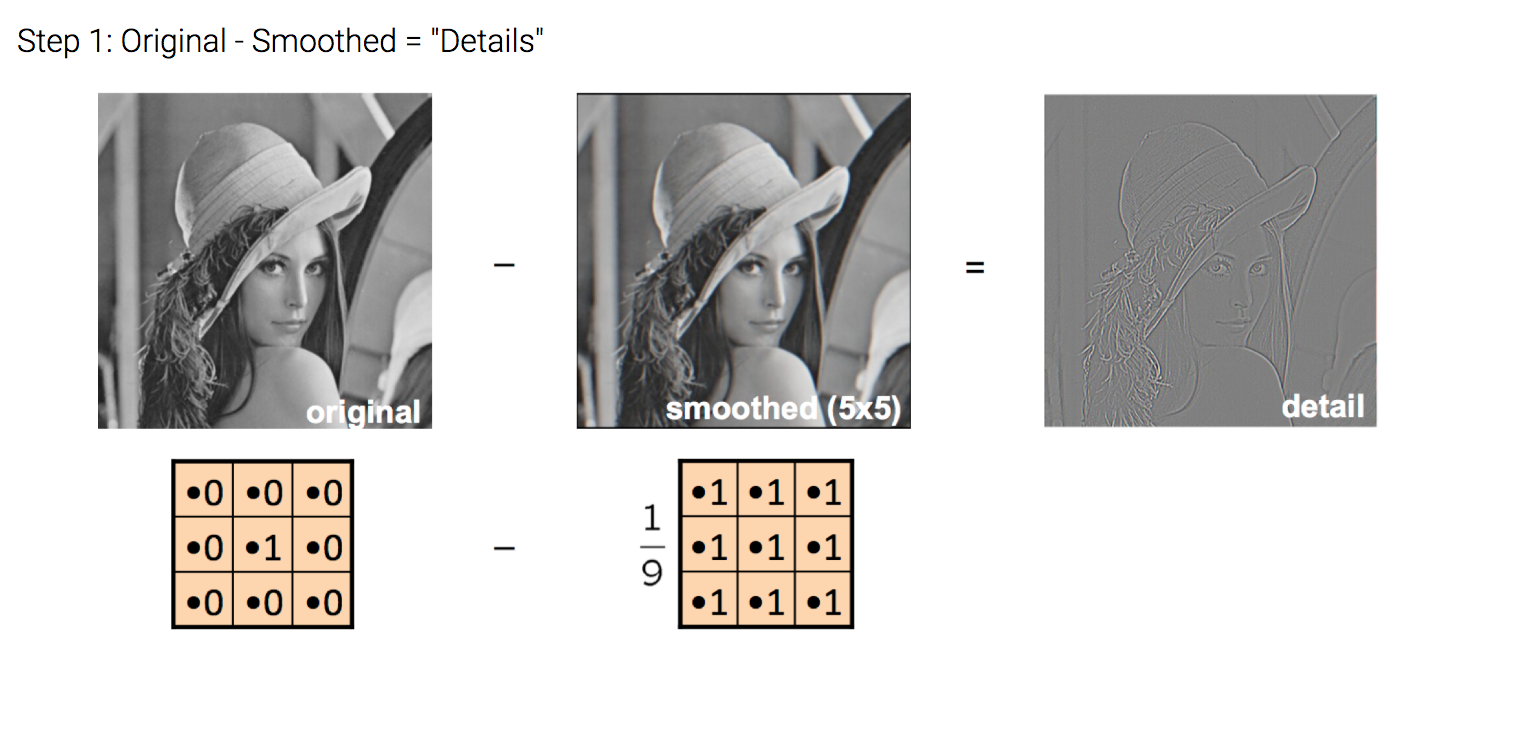
\includegraphics[width=.9\linewidth]{lena_lena_1.png}
\end{center}

\vfill %
\footnotesize
{\color{blue} \url{https://ai.stanford.edu/~syyeung/cvweb/tutorial1.html}}
\end{frame}


\begin{frame}{Можно комбинировать ядра} 
\begin{center}
	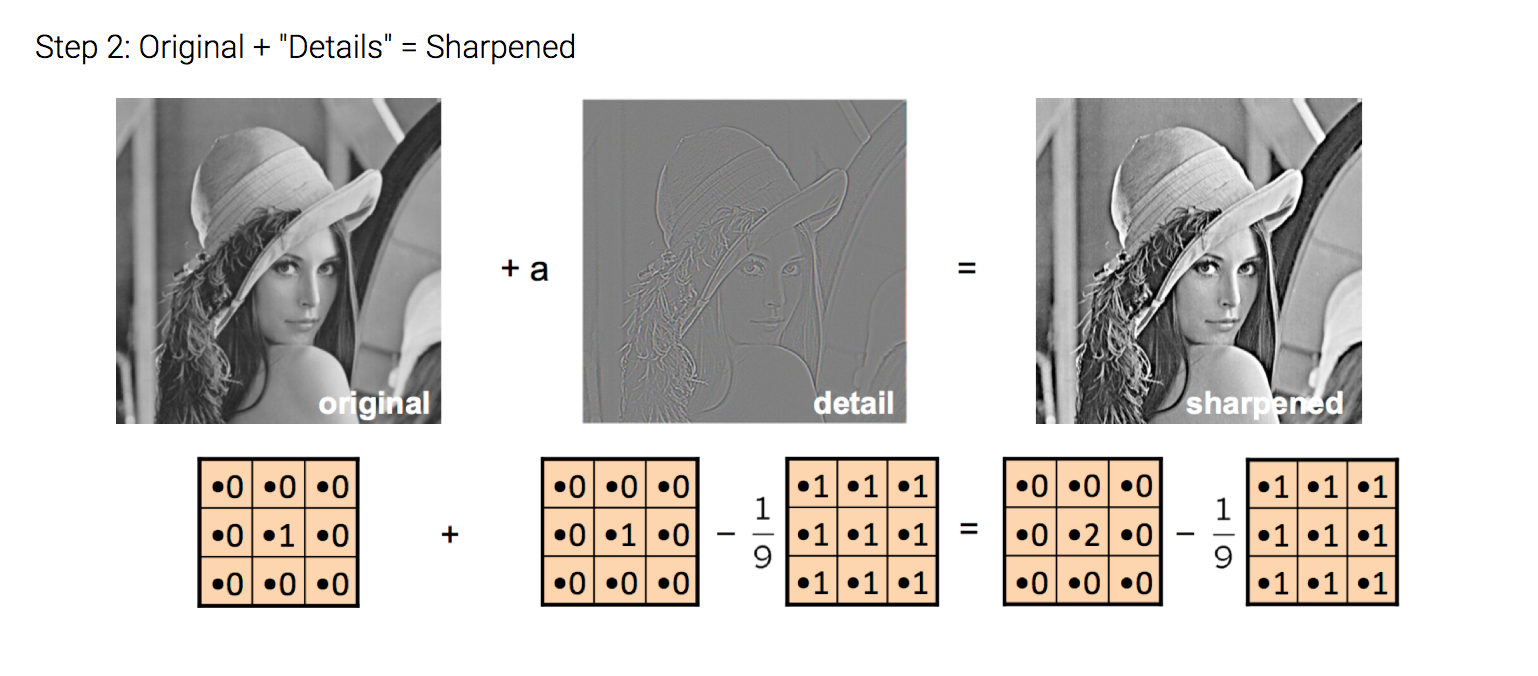
\includegraphics[width=.9\linewidth]{lena_lena_2.png}
\end{center}

\vfill %
\footnotesize
{\color{blue} \url{https://ai.stanford.edu/~syyeung/cvweb/tutorial1.html}}
\end{frame}




\begin{frame}{Свёртка}
\begin{wideitemize}
	\item  Операция свёртки выявляет наличие на изображении паттерна, который задаётся фильтром
	\item Результат операции свёртки — новое изображение
	\item Чем сильнее на участке изображения представлен паттерн, тем больше будет значение свёртки
	\item \alert{Идея:} дать нейросети возможность самостоятельно придумать ядро для поиска нужных ей паттернов
\end{wideitemize}
\end{frame}


\begin{frame}{Классификатор слэшей}
\begin{center}
	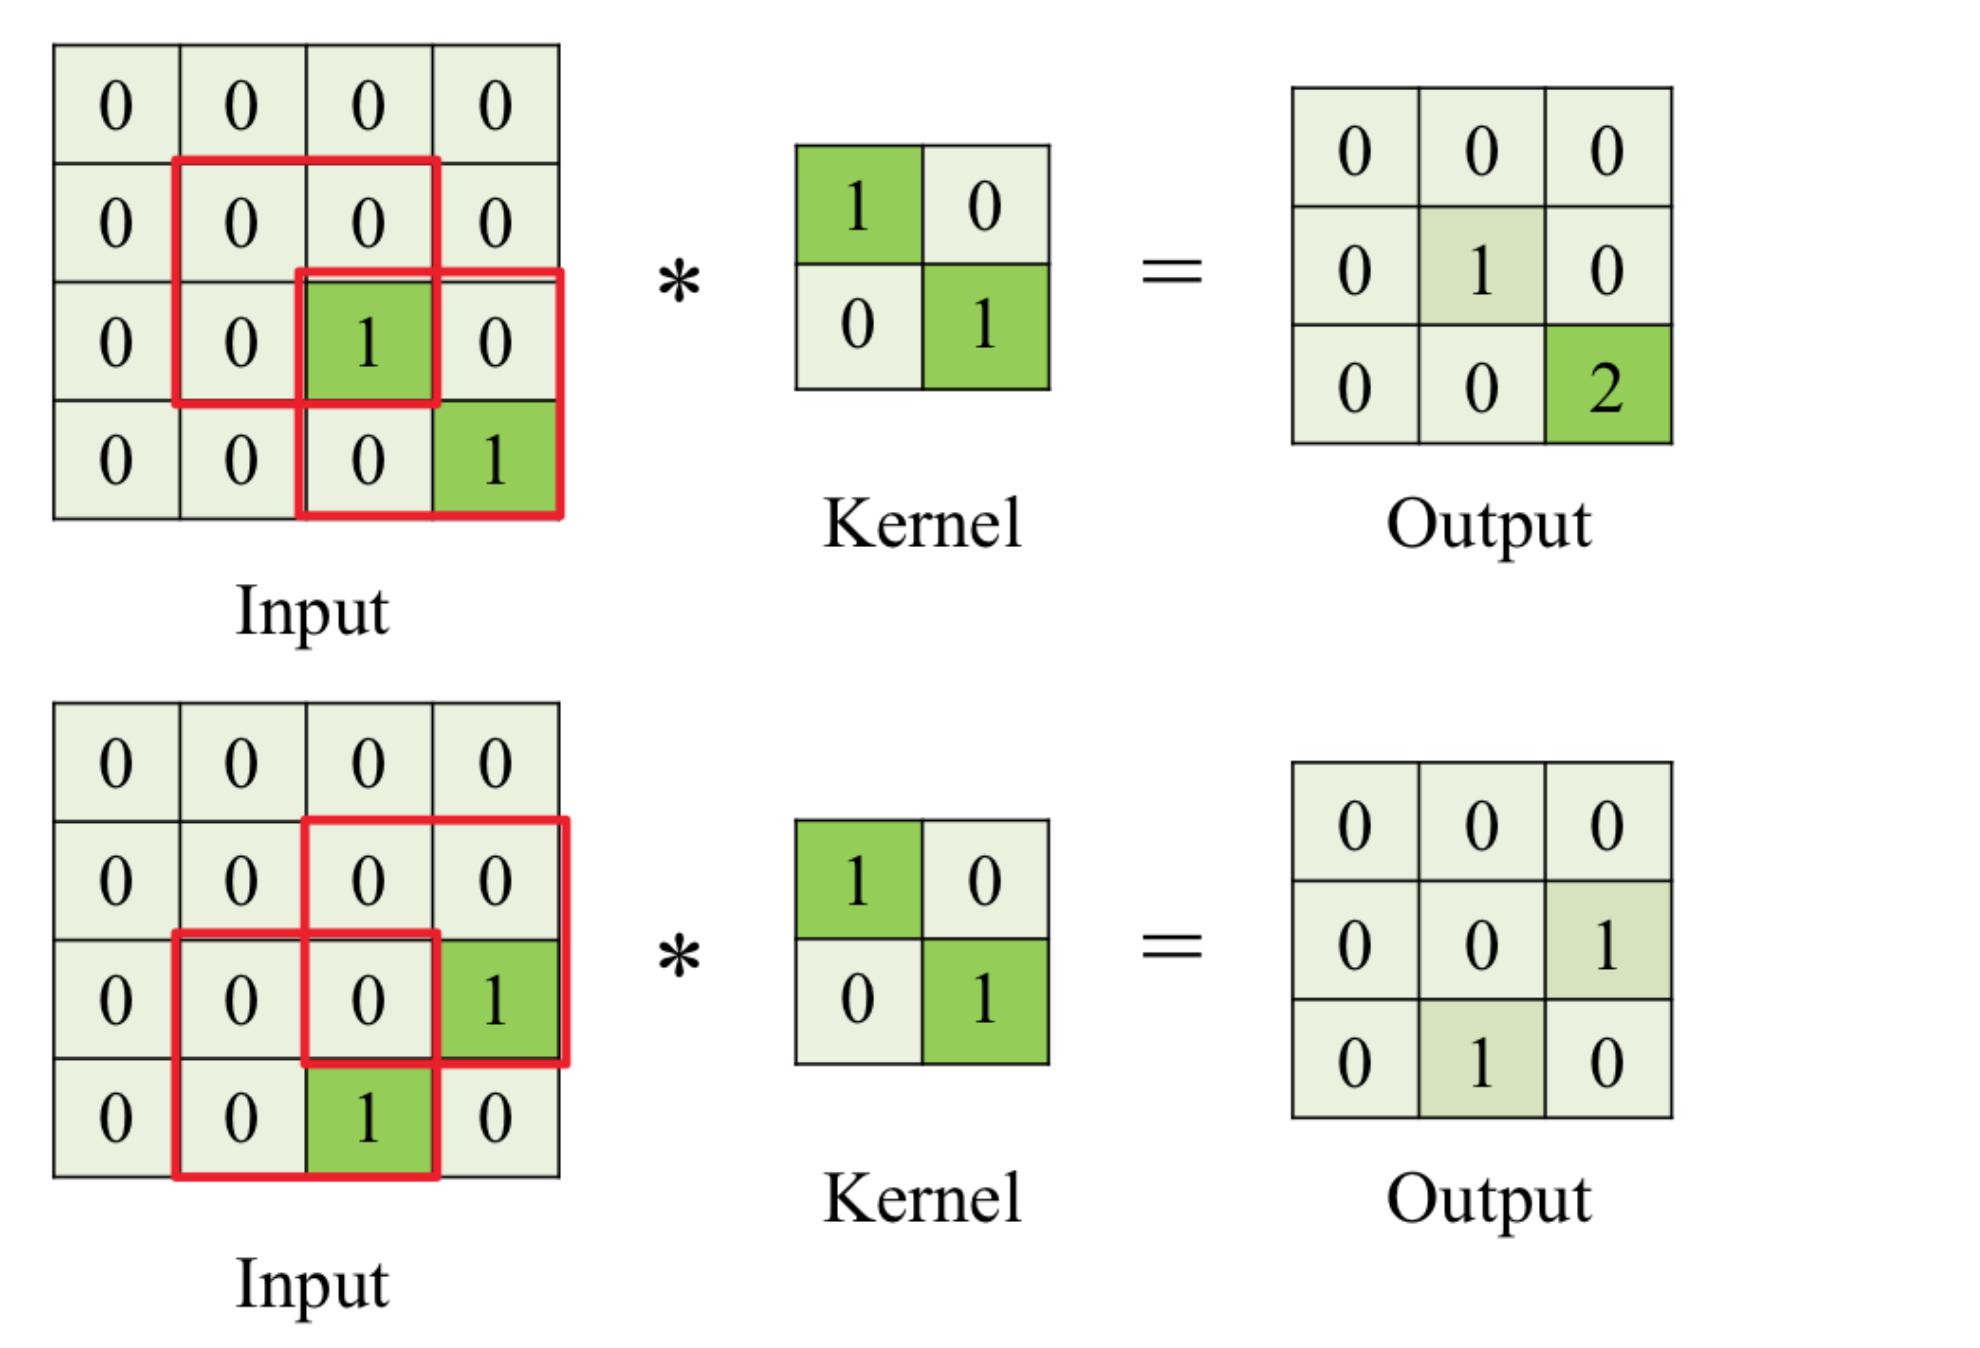
\includegraphics[width=.75\linewidth]{conv_1.png}
\end{center}
\end{frame}


\begin{frame}{Классификатор слэшей}
\begin{center}
	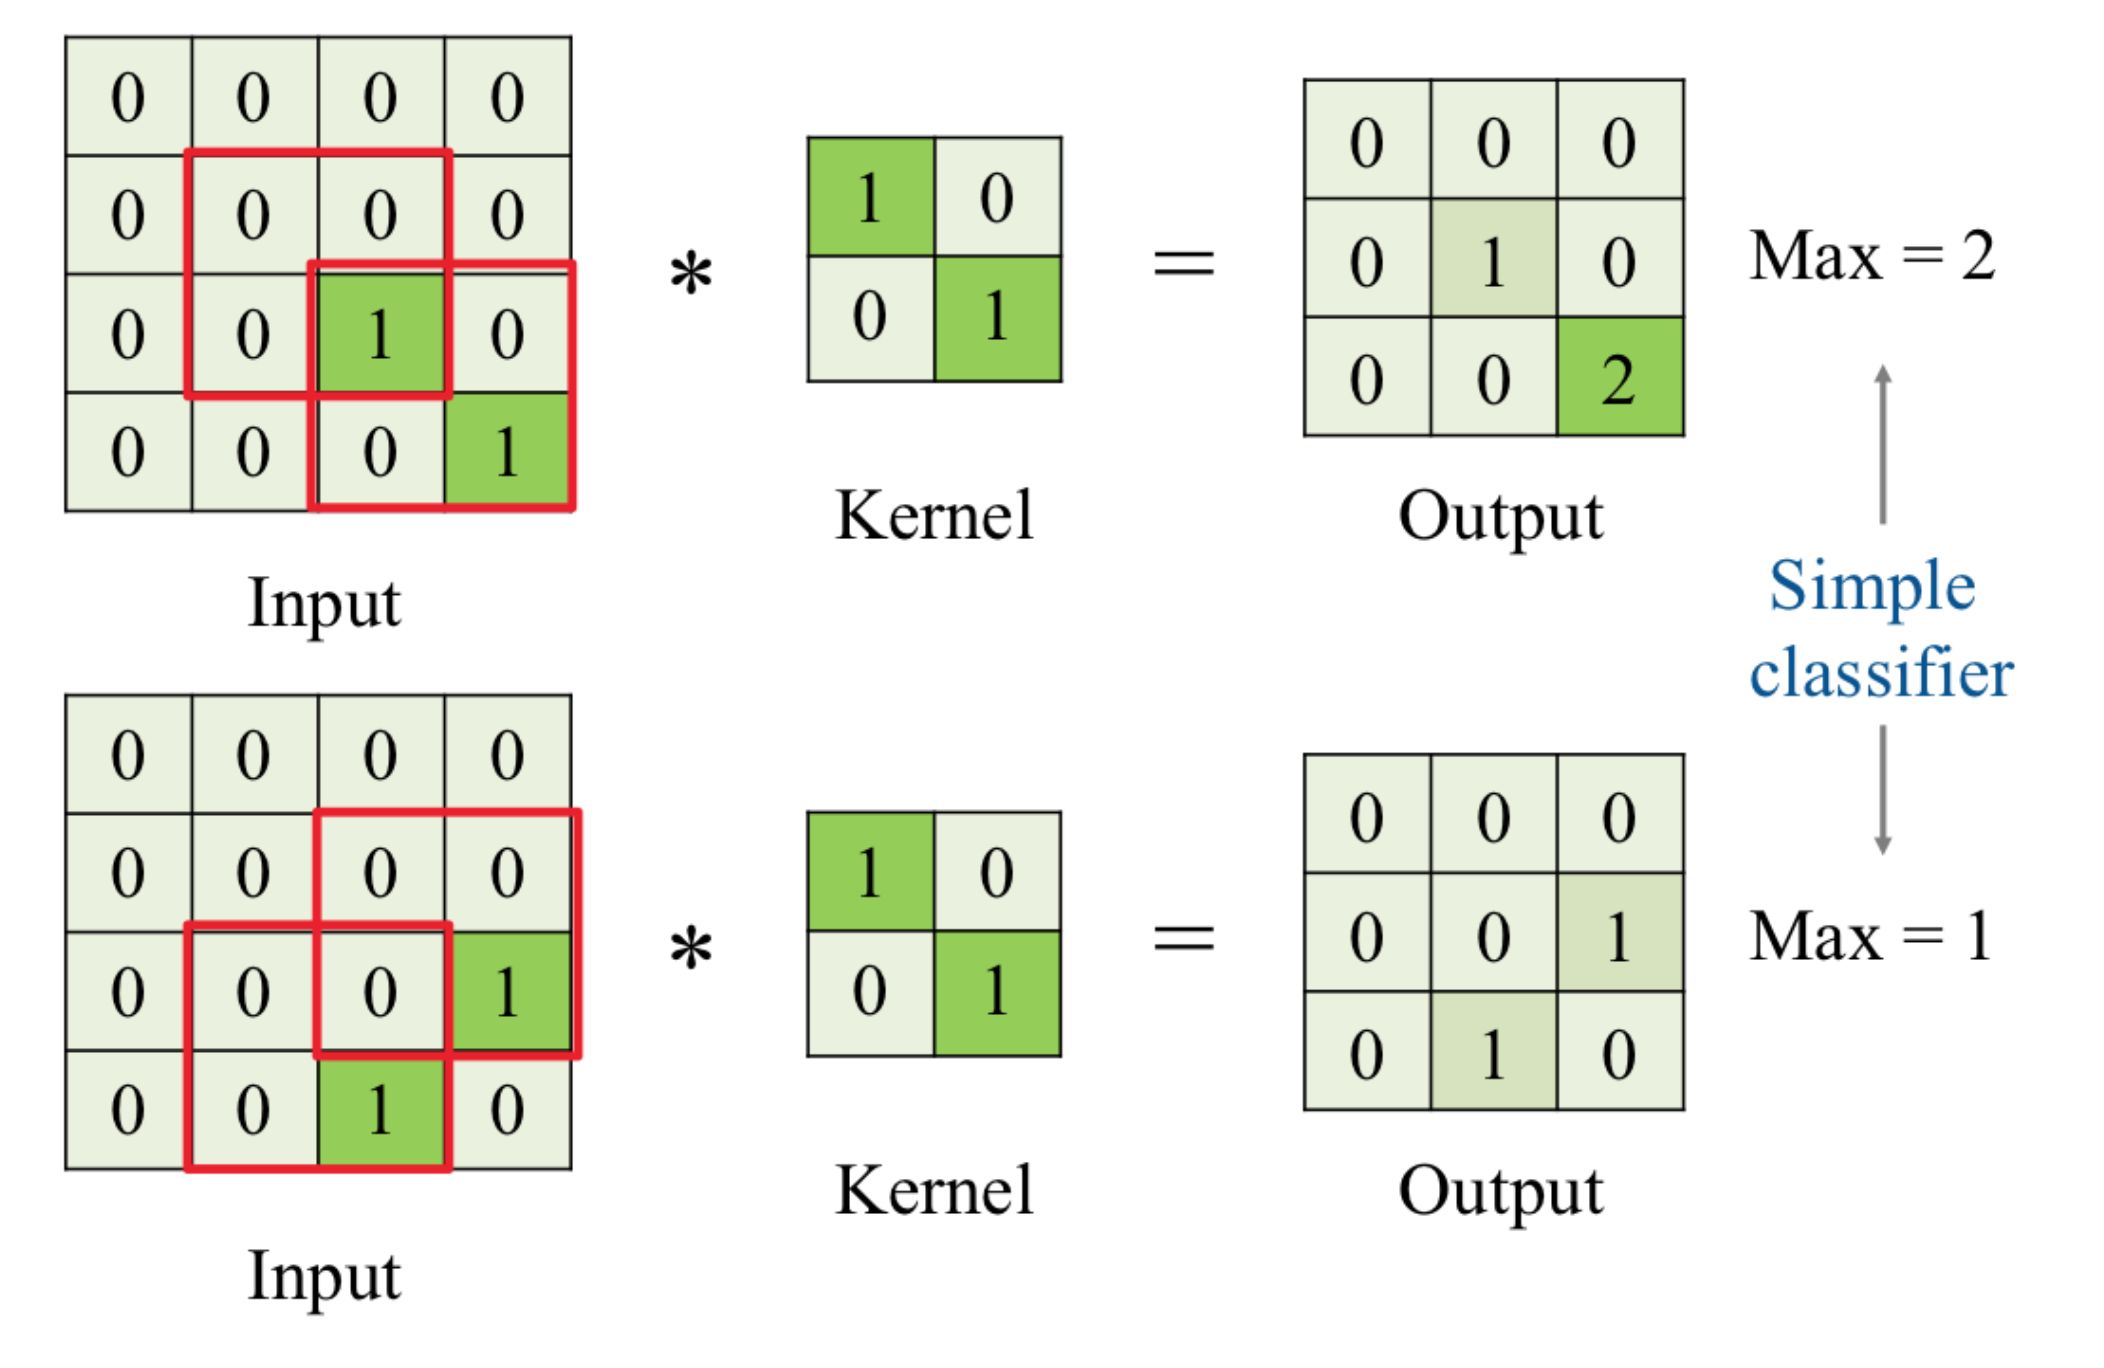
\includegraphics[width=.8\linewidth]{conv_2.png}
\end{center}
\end{frame}


\begin{frame}{Свёртка инвариантна к расположению}
\begin{center}
	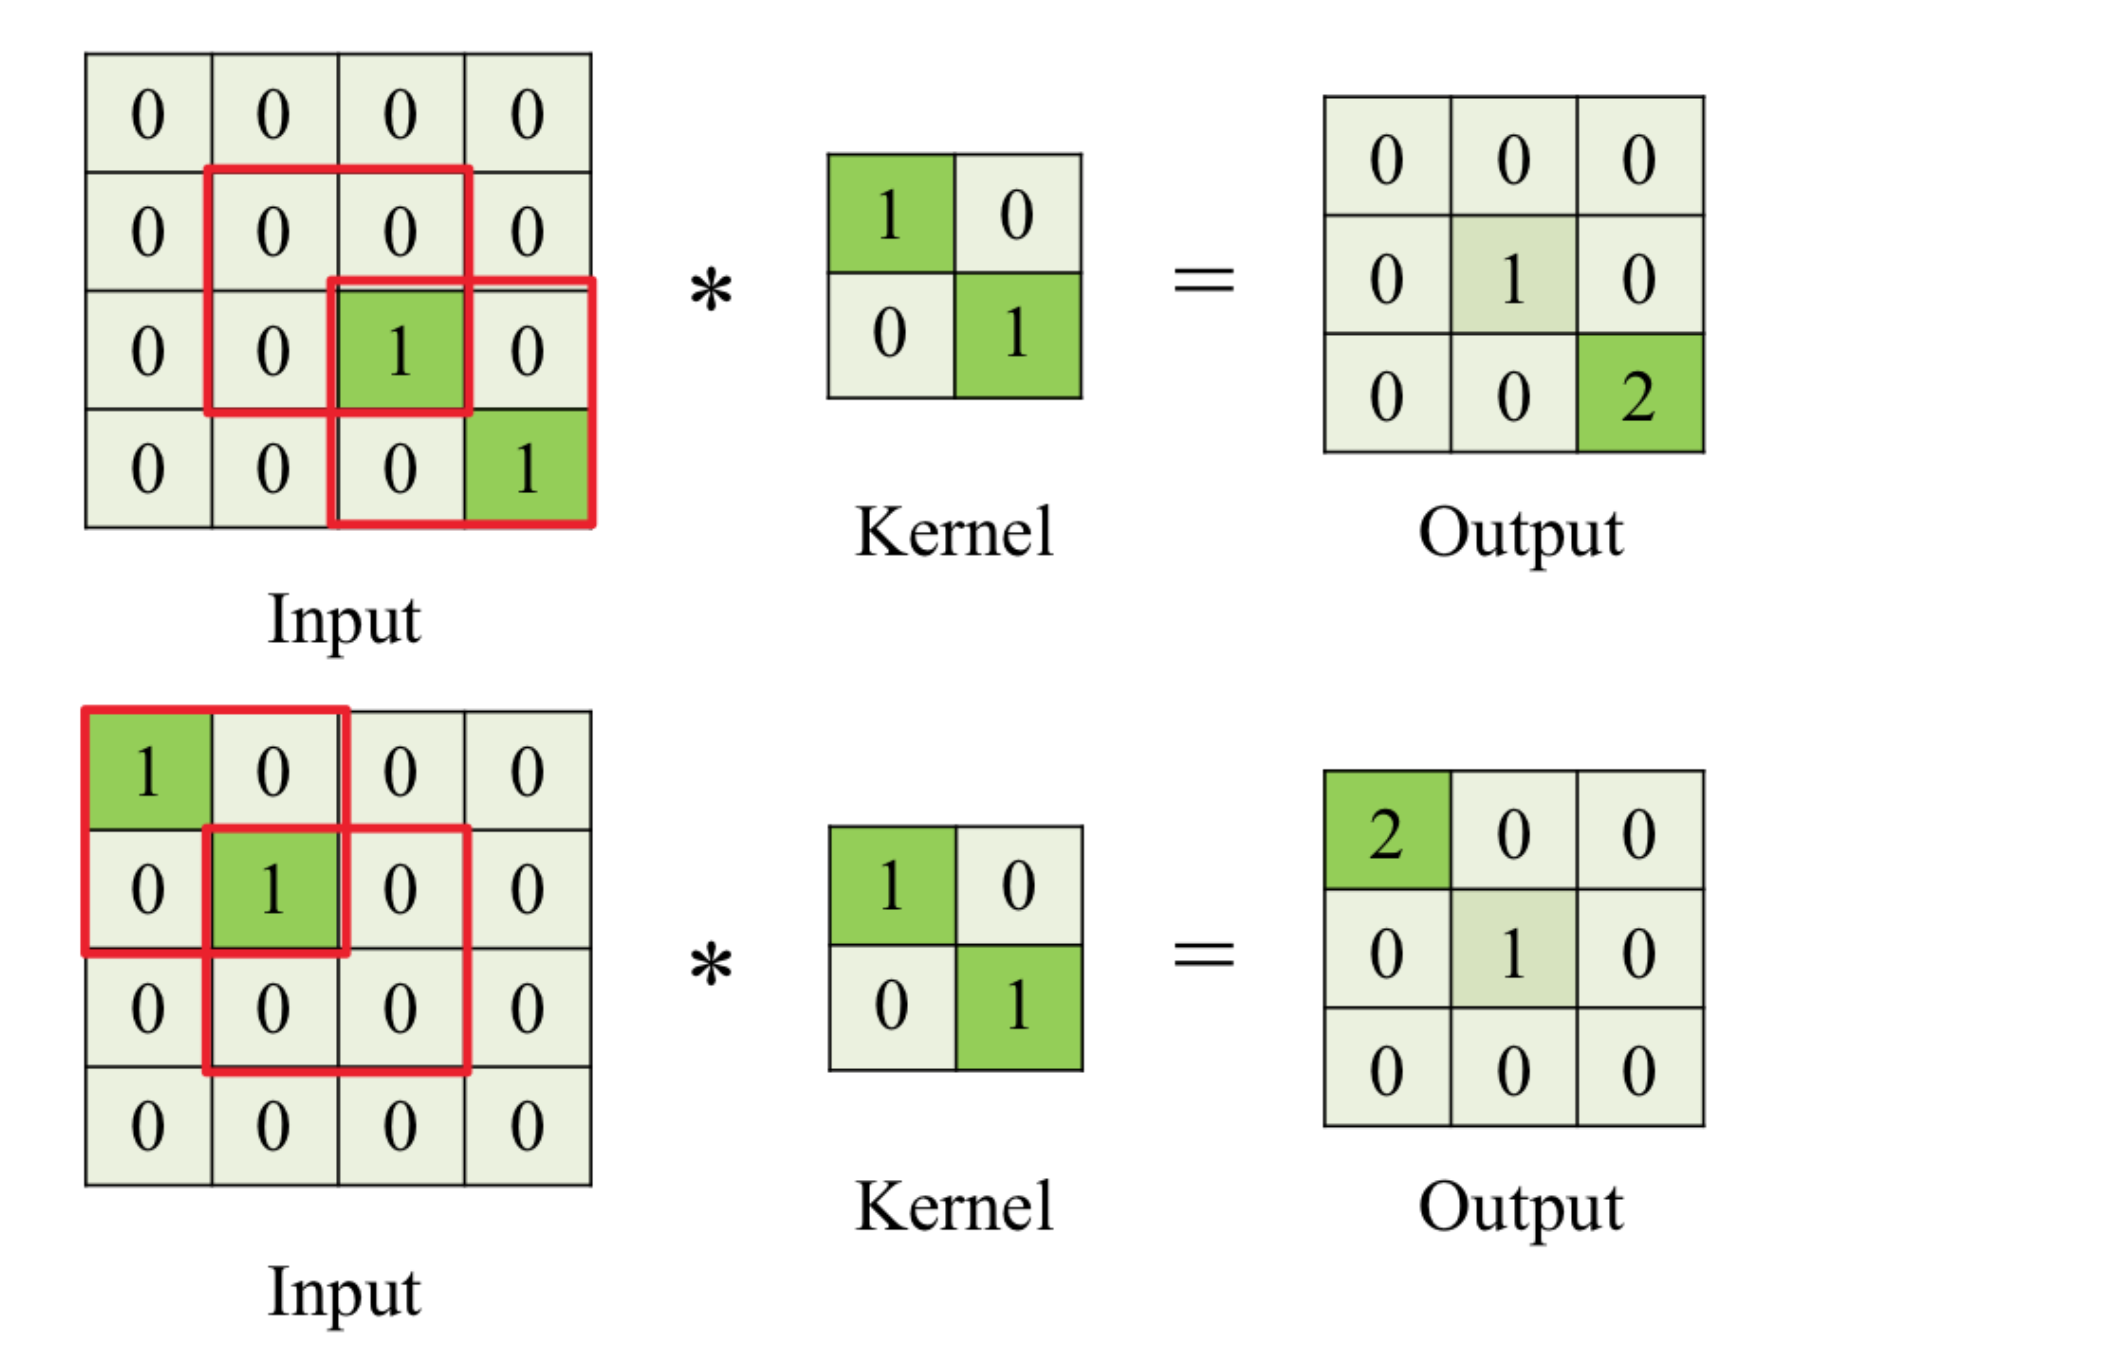
\includegraphics[width=.8\linewidth]{conv_3.png}
\end{center}
\end{frame}


\begin{frame}{Свёртка инвариантна к расположению}
\begin{center}
	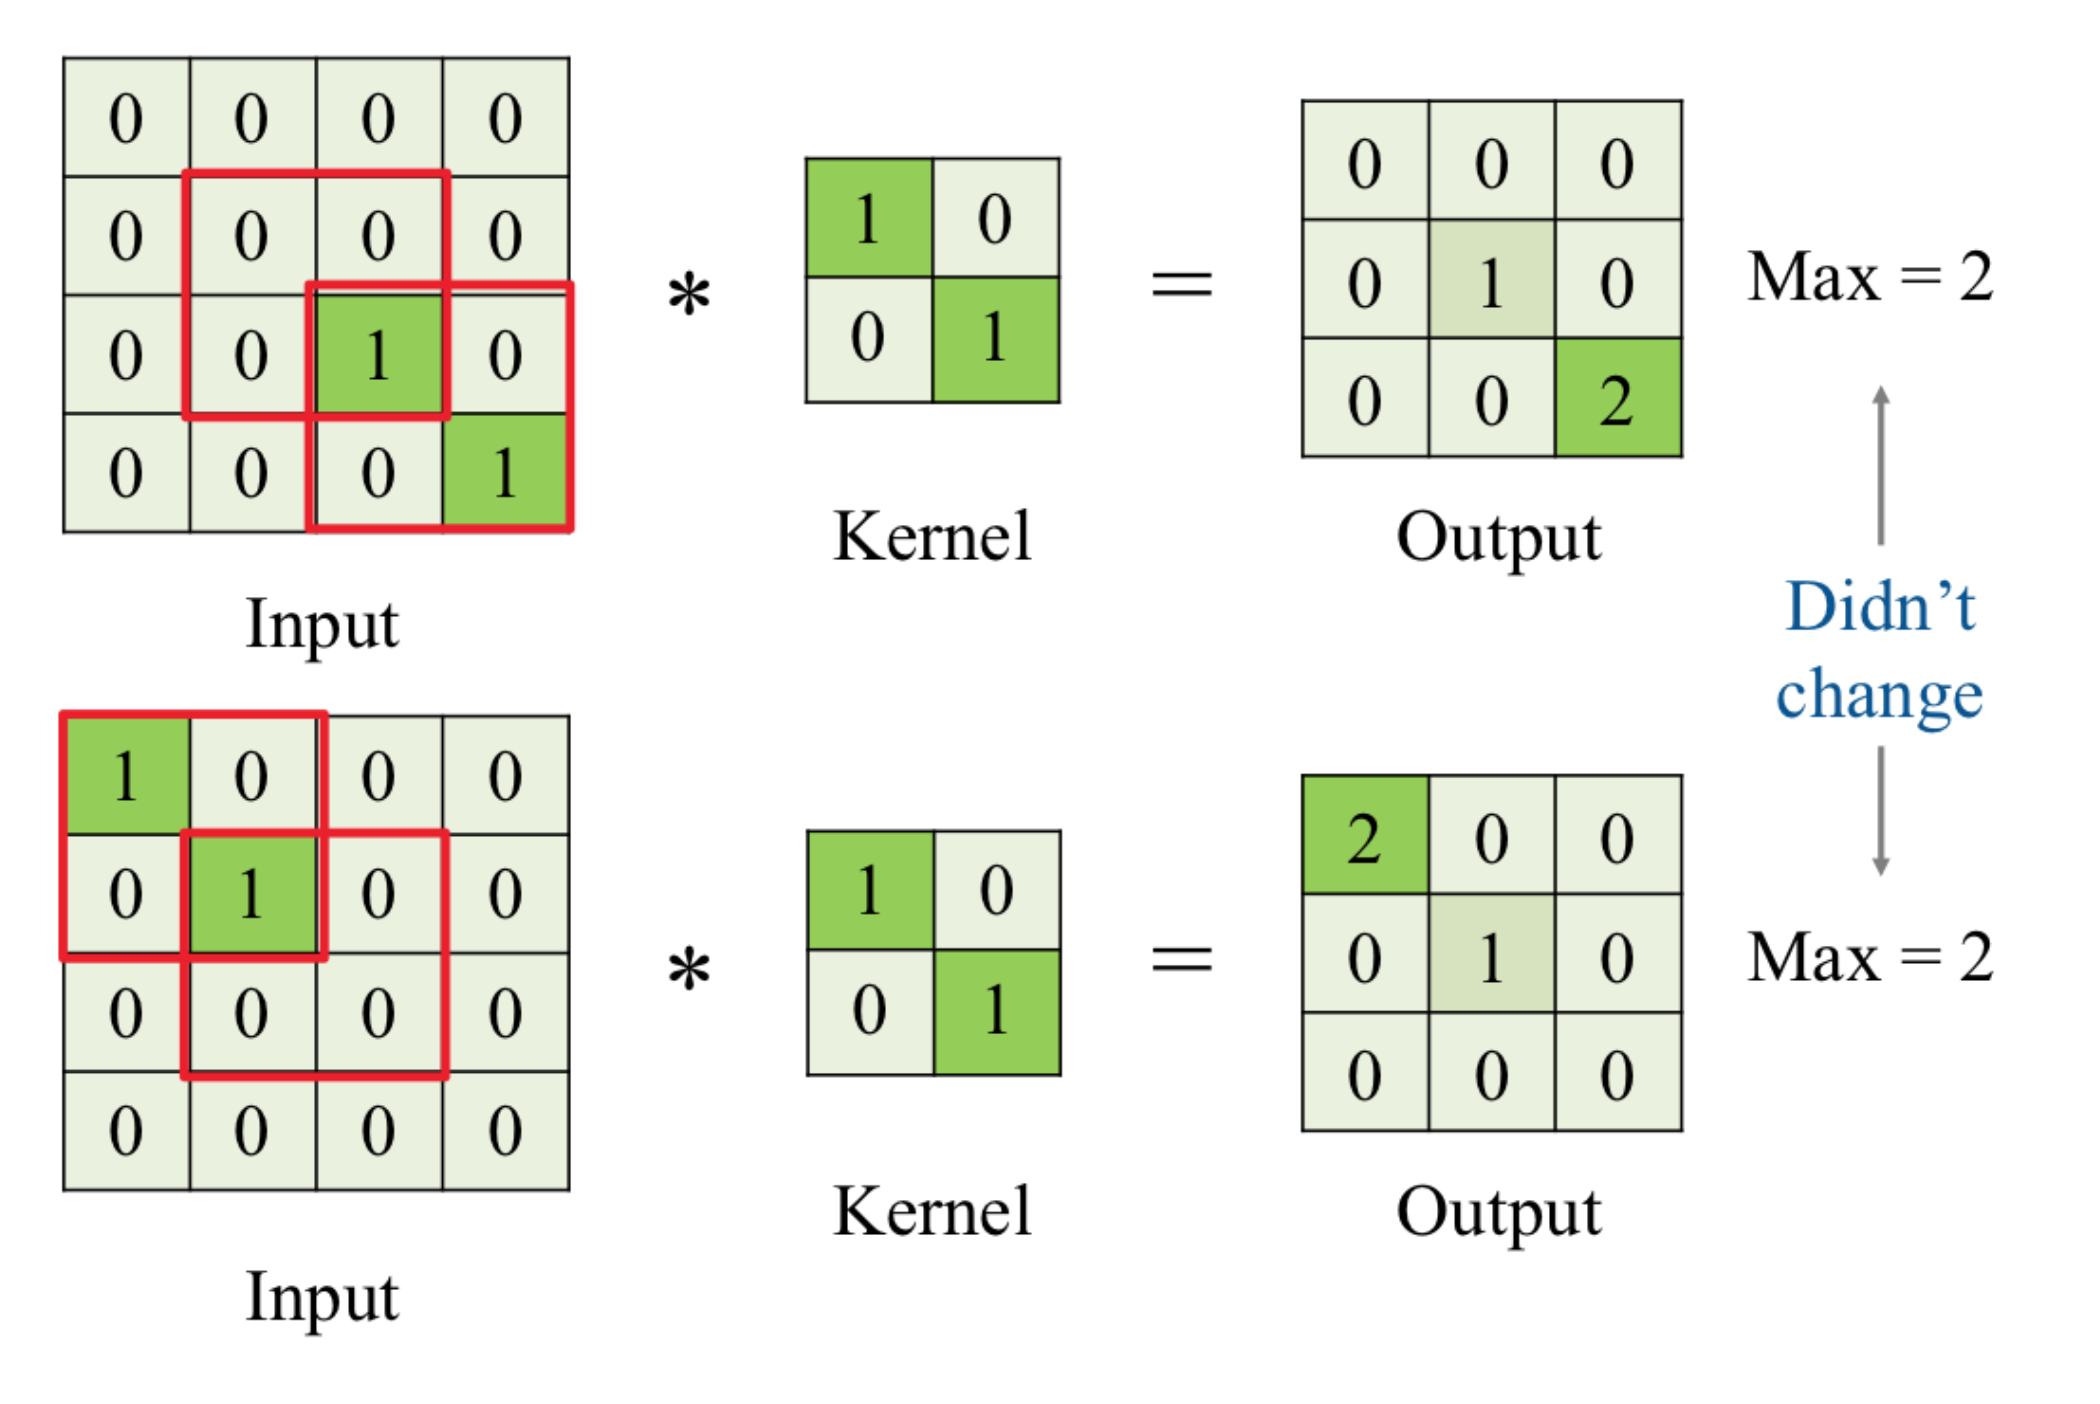
\includegraphics[width=.8\linewidth]{conv_4.png}
\end{center}
\end{frame}


\begin{frame}{Размерность изображения падает}
\begin{center}
	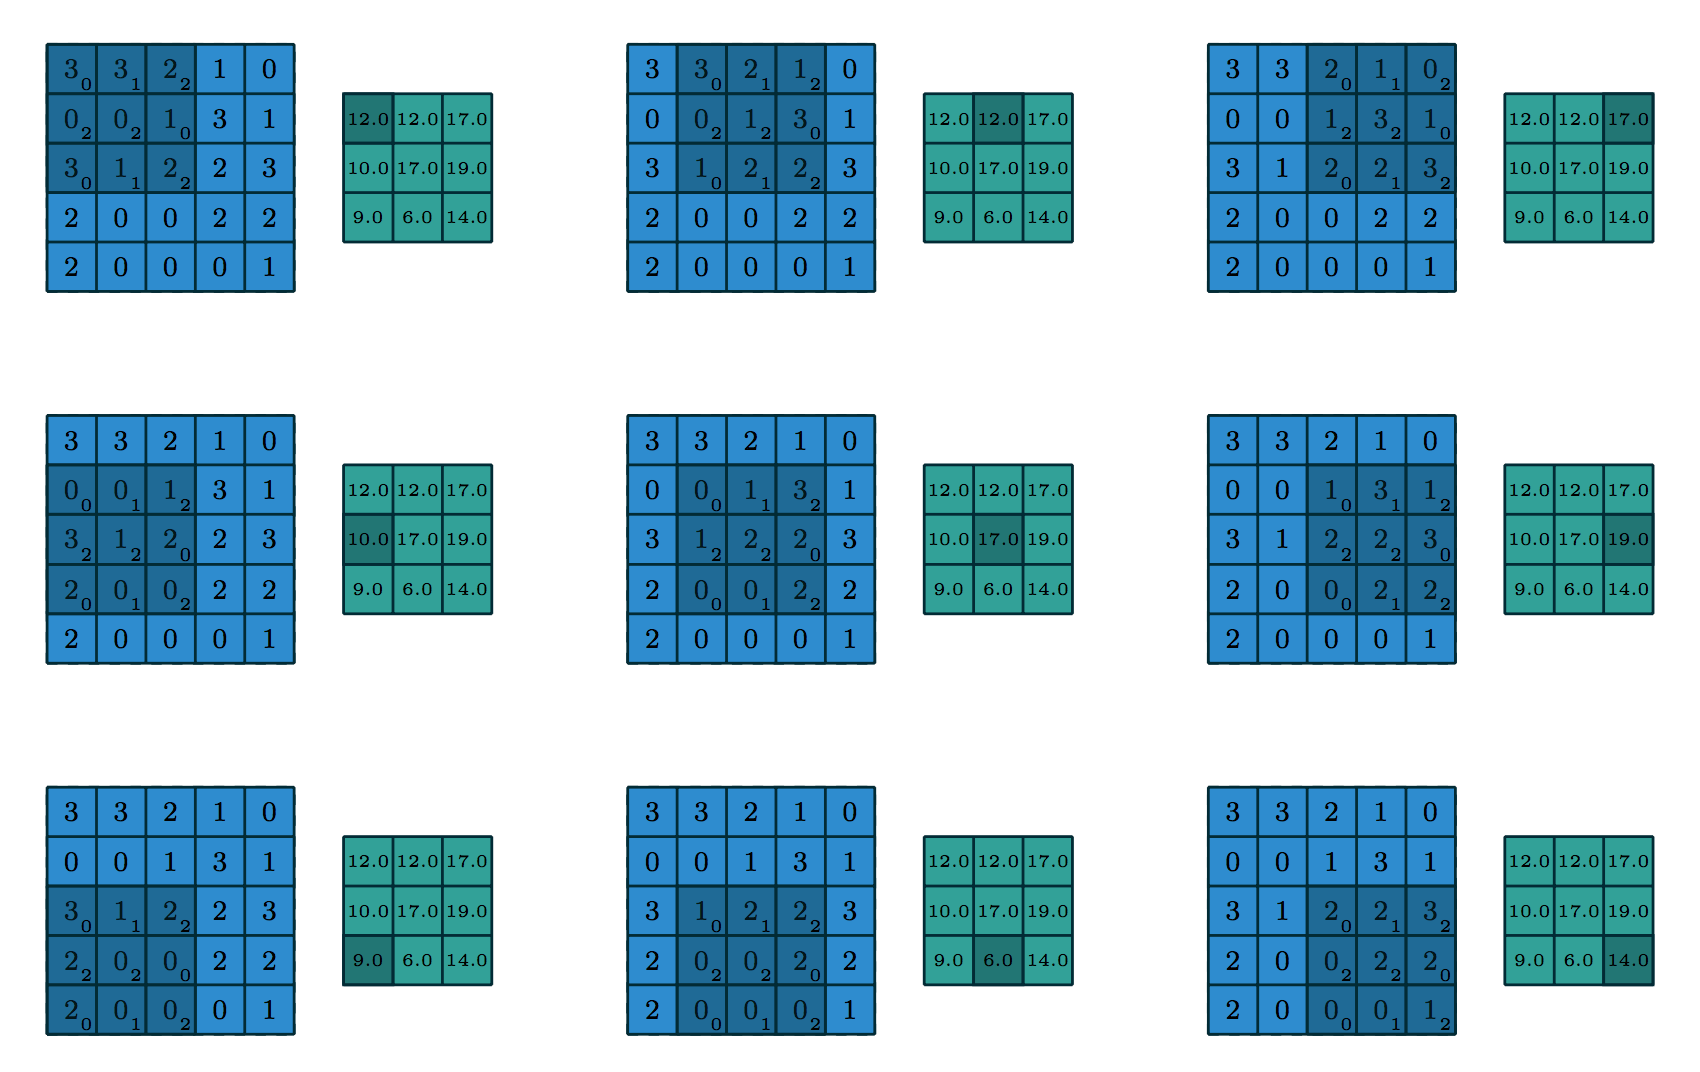
\includegraphics[width=.8\linewidth]{step_by_step_conv.png}
\end{center}

\vfill %
\footnotesize
Хорошее введение в арифметику свёрток: {\color{blue} \url{https://arxiv.org/pdf/1603.07285.pdf}}
\end{frame}


\begin{frame}{Дополнение изображения (zero padding)}
\begin{center}
	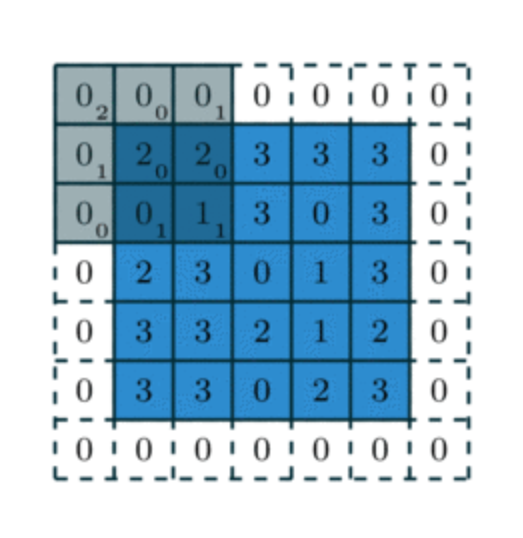
\includegraphics[width=.4\linewidth]{padding.png}
\end{center}
\end{frame}


\begin{frame}{Дополнение (Padding)}
\begin{wideitemize}
	\item Если применять свёртку по формуле, итоговое изображение будет меньше исходного
	\item Из-за этого мы можем терять информацию на краях изображения
	\item Нужно заполнить края рамочкой: zero padding, replication padding, reflection padding
	\item Есть риск, что модель научится понимать, где на изображении края — можем потерять инвариантность
	\item Разные типы паддингов допускают разные способы переобучения под края
\end{wideitemize}
\end{frame}


\begin{frame}{Свёртка в виде формулы}

Чёрно-белый случай:

\[
out[x, y] = \sum_{i = -d}^{d}  \sum_{j= -d}^{d}   K[i, j] \cdot Image[x + i, y + j]
\]

Цветной случай: 

\[
out[x, y] = \sum_{i = -d}^{d}  \sum_{j= -d}^{d}  \sum_{c= 1}^{C}  K[i, j, c] \cdot Image[x + i, y + j, c]
\]

\end{frame}


\begin{frame}{Свёртка для цветной картинки}
\begin{itemize} 
	\item  Цветная картинка — это тензор $W \times H \times C_{in}$
	\item $W$ — высота, $H$ — ширина, $C_{in}$ — число каналов 
\end{itemize}
\begin{center}
	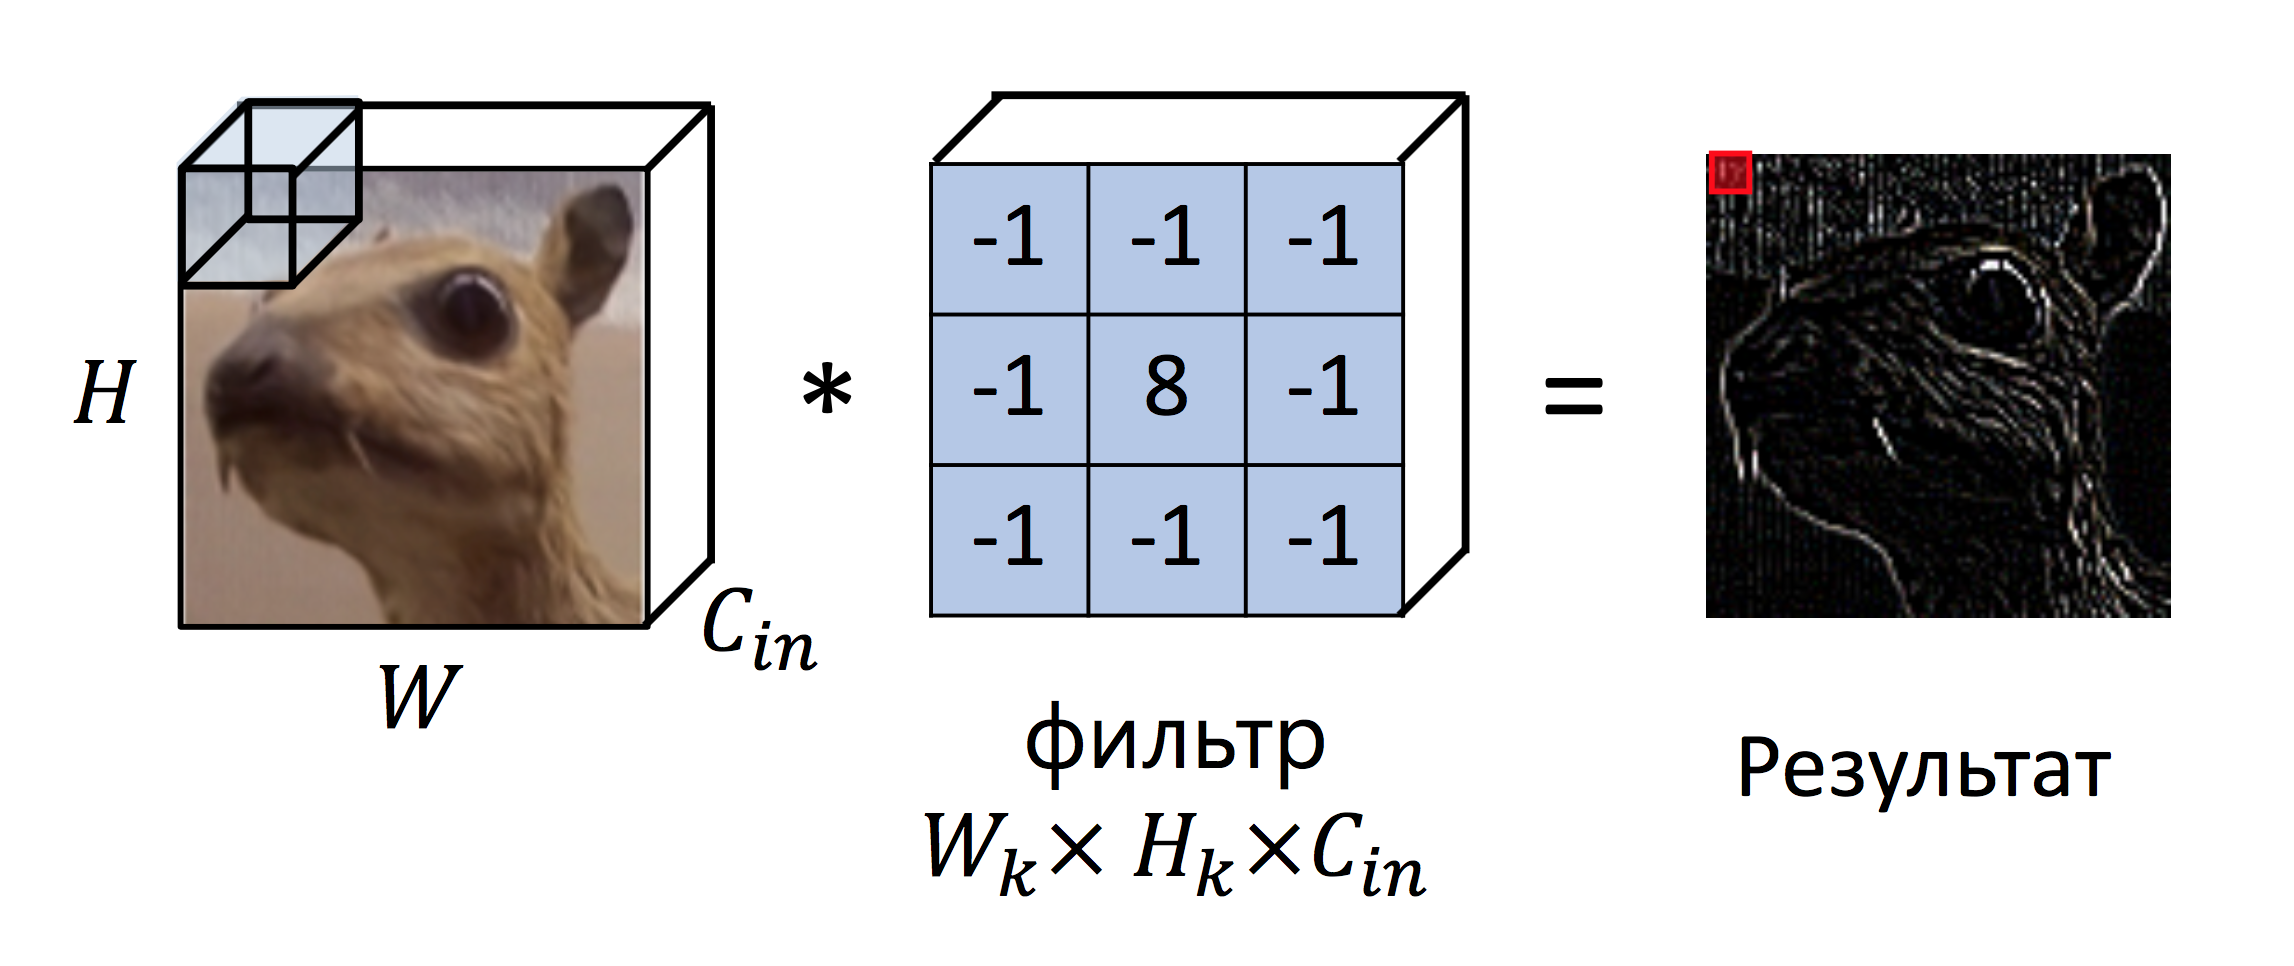
\includegraphics[width=.6\linewidth]{cconv_4.png}
\end{center}
\end{frame}


\begin{frame}{Резюме по свёрткам}
\begin{wideitemize}
	\item Операция свёртки выявляет наличие на изображение паттерна, который задаётся конкретным фильтром (ядром)
	\item Чем сильнее на участке изображения представлен паттерн, тем больше будет значение свёртки 
	\item Результат свёртки изображения с фильтром — новое изображение
	\item Нас будет интересовать много различных паттернов $\Rightarrow$  будем использовать несколько свёрток сразу
\end{wideitemize}

\vfill %
\footnotesize
Хорошее введение в арифметику свёрток: {\color{blue} \url{https://arxiv.org/pdf/1603.07285.pdf}}
\end{frame}



\begin{transitionframe}
	\begin{center}
		\Huge Свёрточный слой
	\end{center}
\centering 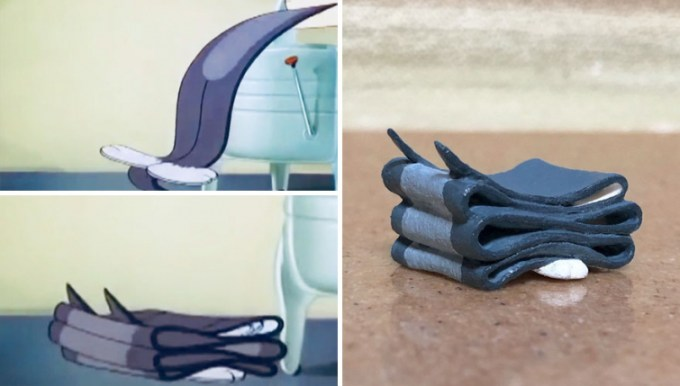
\includegraphics[scale = 0.18]{conv_tom2.jpg}
\end{transitionframe}


\begin{frame}{Свёрточный слой}
\alert{Идея:} дать нейросети возможность самостоятельно придумать ядро для поиска нужных ей паттернов
\end{frame}


\begin{frame}{Свёрточный слой}
\begin{center}
	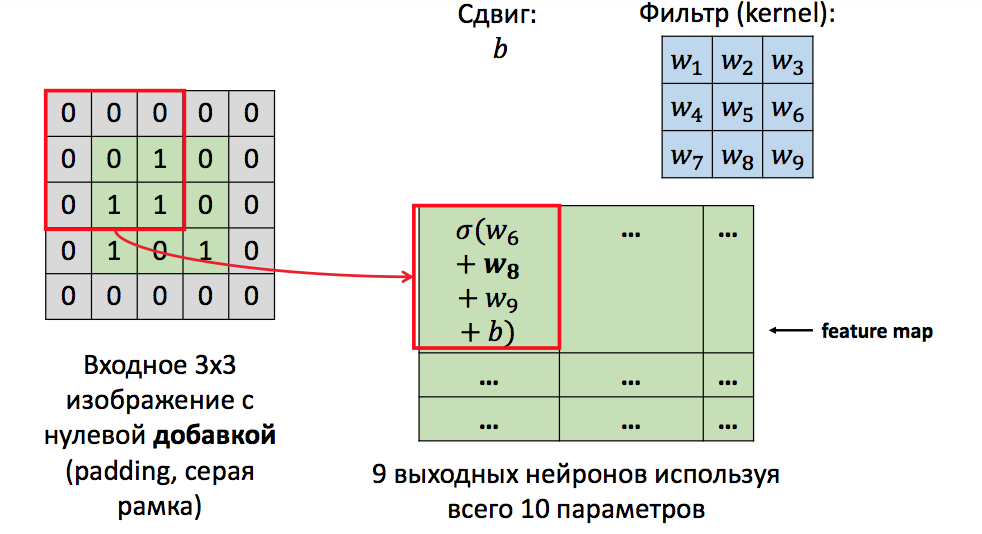
\includegraphics[width=.8\linewidth]{conv_layer.png}
\end{center}
\end{frame}


\begin{frame}{Свёрточный слой}
\begin{center}
	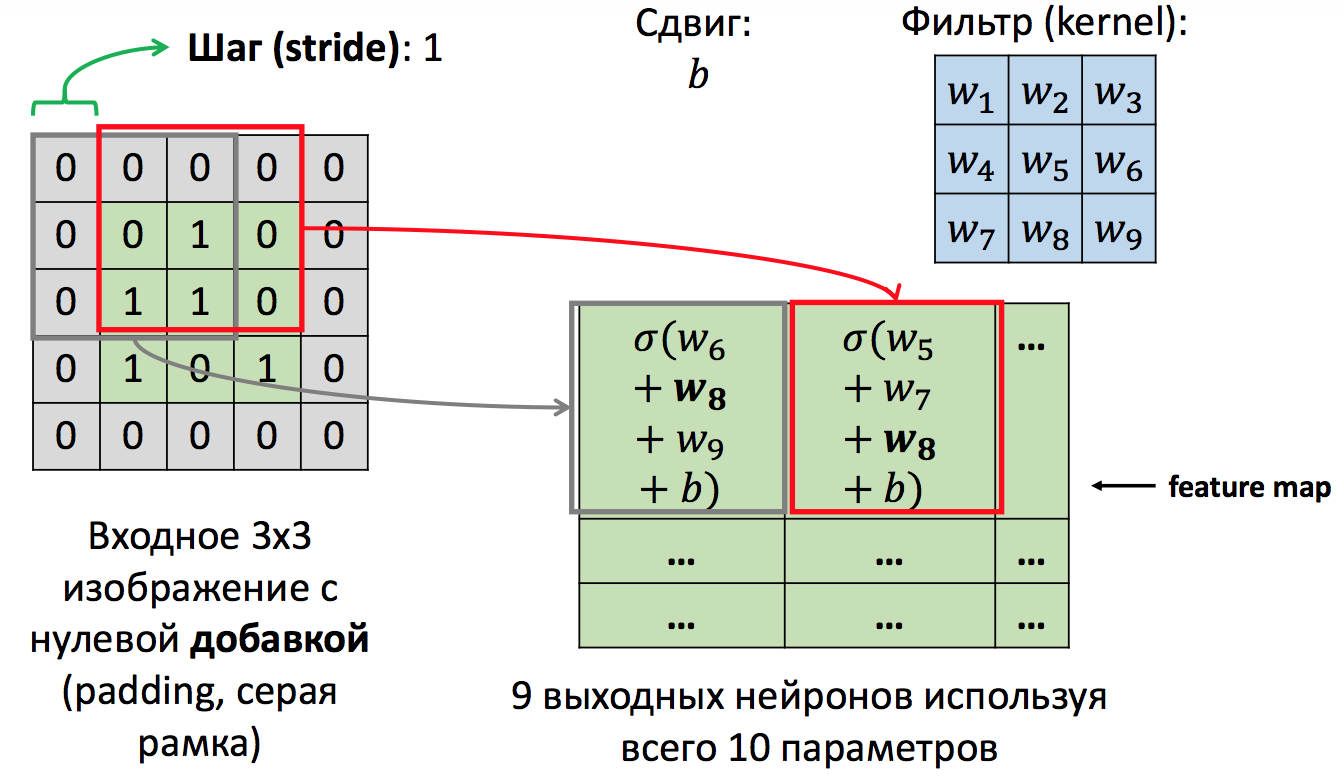
\includegraphics[width=.8\linewidth]{conv_layer_2.png}
\end{center}
\end{frame}


\begin{frame}{Как считать градиенты}
\begin{center}
 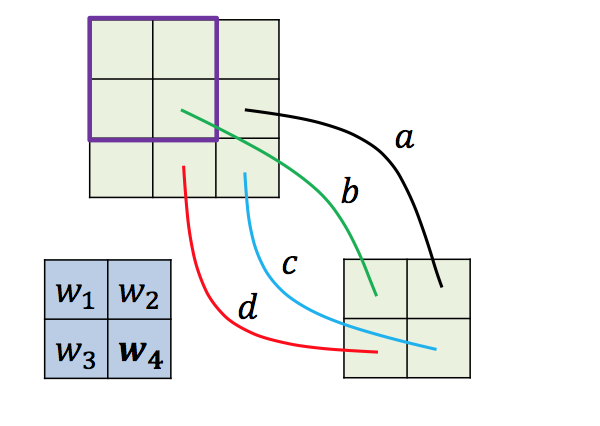
\includegraphics[width=.4\linewidth]{back_cl1.png}
\end{center}

\only<1>{
	\begin{equation*}
	\begin{aligned}
	& b = w_1 x_{11} + w_2 x_{12} + w_3 x_{21} + w_4 x_{22} \\
	& a = w_1 x_{12} + w_2 x_{13} + w_3 x_{22} + w_4 x_{23} 
	\end{aligned}
	\end{equation*}
}

\only<2-3>{
	\[
	\frac{\partial L}{\partial w_1} = \frac{ \partial L }{\partial a} \cdot x_{11} + \frac{ \partial L }{\partial b} \cdot x_{12} + \frac{ \partial L }{\partial c} \cdot x_{21}  + \frac{ \partial L }{\partial d} \cdot x_{22} 
	\]
}

\only<3>{Суммируем градиенты по всем использованиям веса $w_4$ }
\end{frame}


\begin{frame}{Свёрточный слой}
\begin{wideitemize}
	\item  Слой действует одинаково для каждого участка картинки, в отличие от полносвязного 
	\item  Нужно оценивать меньшее количество параметров
	\item  Слой учитывает взаимное расположение пикселей
	\item  Можно учить тем же самым алгоритмом обратного распространения ошибки
	\item  Свёрточный слой —  это полносвязный слой с ограничениями
\end{wideitemize}
\end{frame}


\begin{frame}{В свёрточном слое меньше параметров}
\begin{wideitemize}
	\item  Картинка $300 \times 300$
	\item  $300 \times 300$  нейронов
	\item  Свертка $5 \times 5$ – $26$ параметров
	\item В полносвязном слое – $8.1 \cdot 10^9$ параметров
\end{wideitemize}
\end{frame}


\begin{frame}{Одного фильтра мало!}
\begin{columns}
	\begin{column}{.49\textwidth}
		\begin{wideitemize} 
			\item На входе $W \times H \times C_{in}$
			\item На выходе $W \times H \times C_{out}$
			\item В одном пикселе появляется глубина с разными характеристиками пикселя изображения
			\item \only<1> {\alert{Сколько параметров надо оценить?}}  \only<2> {$(W_k \cdot H_k \cdot C_{in} + 1) \cdot C_{out}$}
		\end{wideitemize}
	\end{column}
	\begin{column}{.49\textwidth}
		\begin{center}
			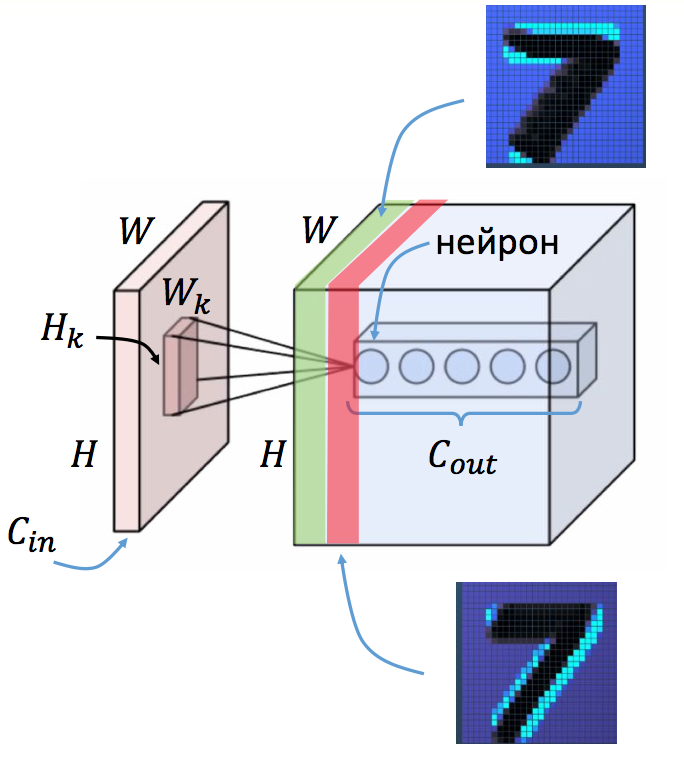
\includegraphics[width=.9\linewidth]{convolution3.png}
		\end{center}
	\end{column}
\end{columns}
\end{frame}


\begin{frame}{Поле видимости (receptive field)}
\begin{center}
	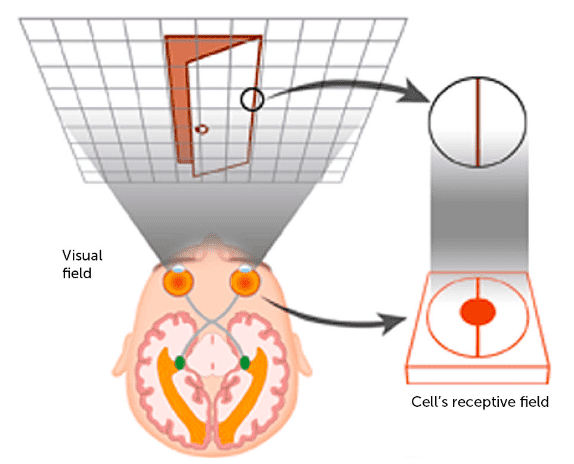
\includegraphics[width=.5\linewidth]{Visual-human-system.png}
\end{center}
\vfill %
\footnotesize
\color{blue} \url{https://theaisummer.com/receptive-field/}
\end{frame}


\begin{frame}{Поле видимости (receptive field)}
\begin{center}
	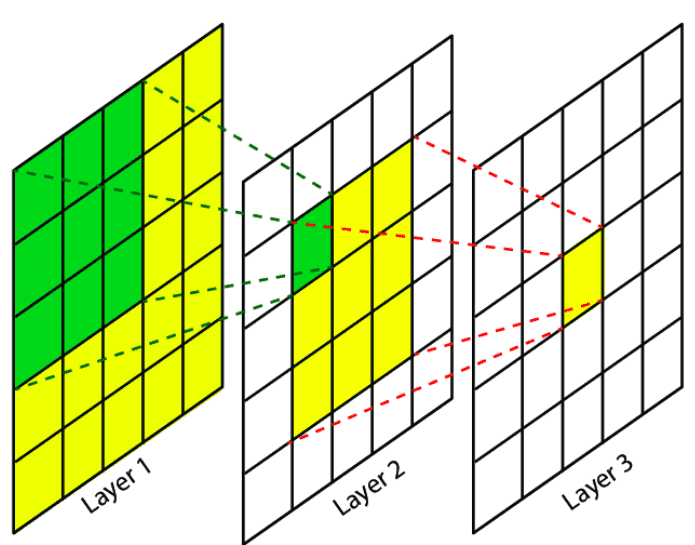
\includegraphics[width=.5\linewidth]{receptive-field-in-convolutional-networks.png}
\end{center}
\vfill %
\footnotesize
\color{blue} \url{https://theaisummer.com/receptive-field/}
\end{frame}


\begin{frame}{Одного свёрточного слоя недостаточно}
\begin{wideitemize}
	\item  Нейроны первого слоя смотрят на поле $3 \times 3$ 
	\item  Если интересующий нас объект больше, нам нужна вторая свёртка 
\end{wideitemize}

\begin{center}
	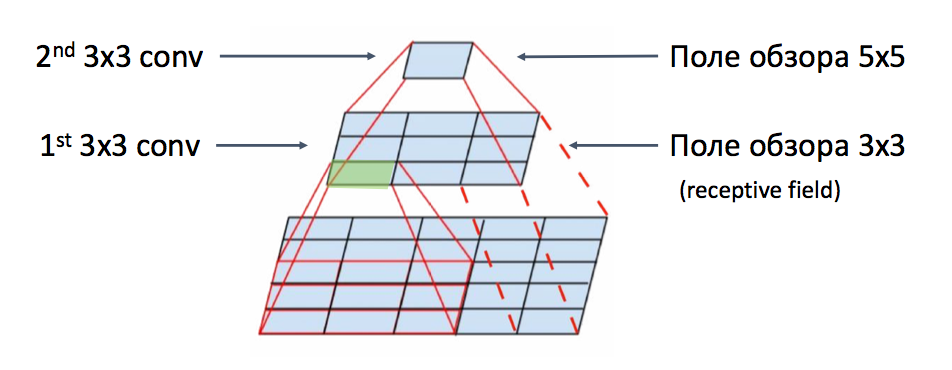
\includegraphics[width=.8\linewidth]{rec_field.png}
\end{center}
\end{frame}


\begin{frame}{Одного свёрточного слоя недостаточно}
\begin{wideitemize}
\item  $N$ слоёв со свёртками $3 \times 3$ 
\item  На $N$-ом слое поле обзора  $(2N + 1) \times (2N + 1)$
\item  Если наш объект размера $300 \times 300$, надо $150$ слоёв... 
\end{wideitemize}

\begin{center}
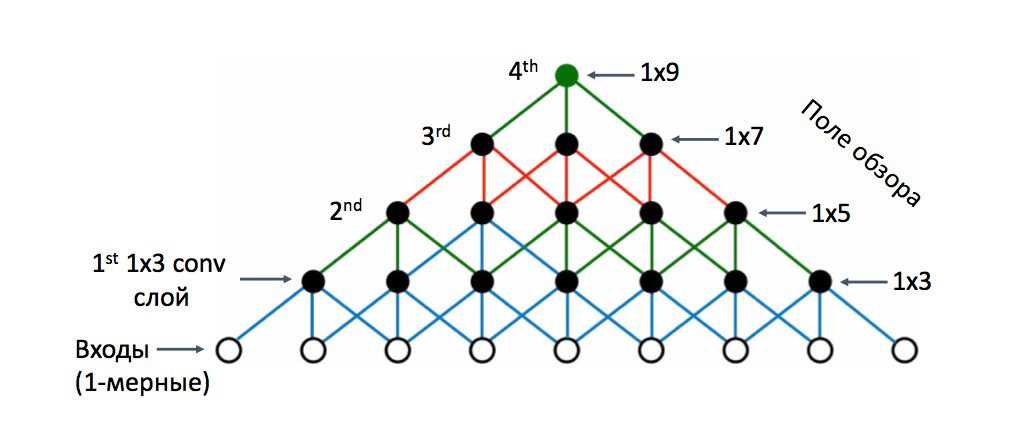
\includegraphics[width=.8\linewidth]{rec_field2.png}
\end{center}
\end{frame}


\begin{frame}{Помоги CNN найти машину}
\begin{wideitemize}
	\item Наша цель - детекция автомобилей	
	\item  Оранжевым и зелёным выделены два разных поля видимости
	\item  \alert{Сеть с маленьким полем видимости не сможет распознать машину} 
\end{wideitemize}

\begin{center}
	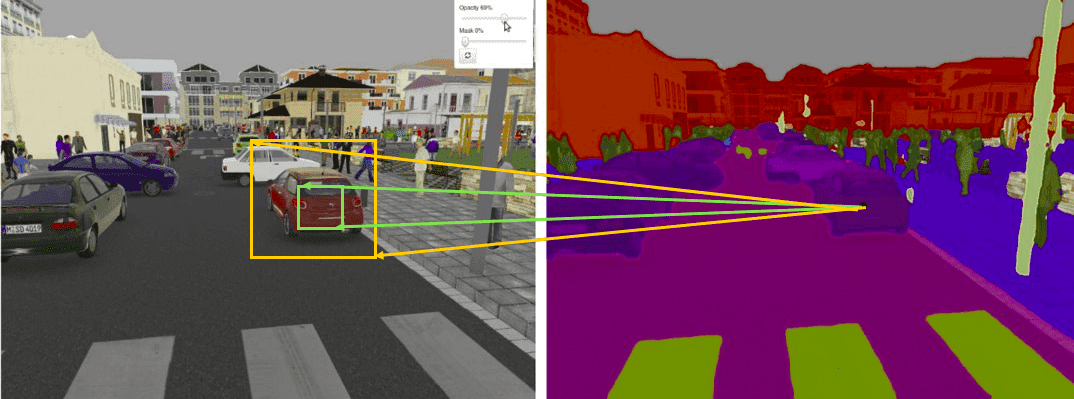
\includegraphics[width=.7\linewidth]{receptive-fields-semantic-segmentation.png}
\end{center}
\vfill %
\footnotesize
\color{blue} \url{https://theaisummer.com/receptive-field/}
\end{frame}


\begin{frame}{Зависимость точности сети от поля обзора}
\begin{center}
	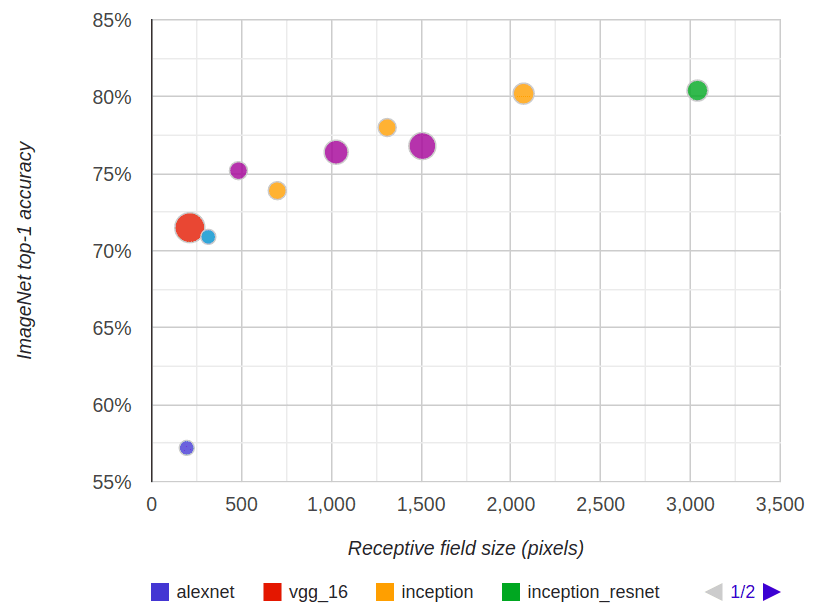
\includegraphics[width=.57\linewidth]{imagenet-classification-and-receptive-field.png}
\end{center}
\vfill %
\footnotesize
\color{blue} \url{https://theaisummer.com/receptive-field/} \newline 
\color{blue} \url{https://distill.pub/2019/computing-receptive-fields/}
\end{frame}



\begin{frame}{Нужно растить поле обзора быстрее!}
\vspace{5mm}
\alert{Можно увеличить шаг свёртки}
	\begin{center}
		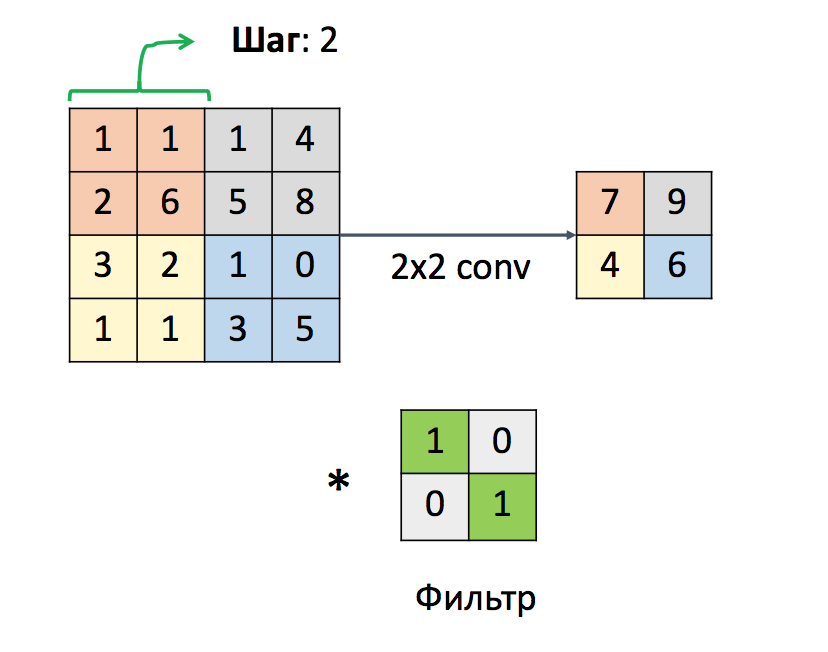
\includegraphics[width=.6\linewidth]{stride_01.png}
	\end{center}
\end{frame}


\begin{frame}{Свёртки с пропусками (strides)}
	\begin{wideitemize}
		\item Пиксели локально скоррелированы — соседние пиксели, как правило, не сильно отличаются друг от друга	
		\item  Если будем делать свёртку с каким-то шагом, не потеряем много информации
		\item  \alert{Очень агрессивная стратегия снижения размерности картинки}
	\end{wideitemize}
	\begin{center}
		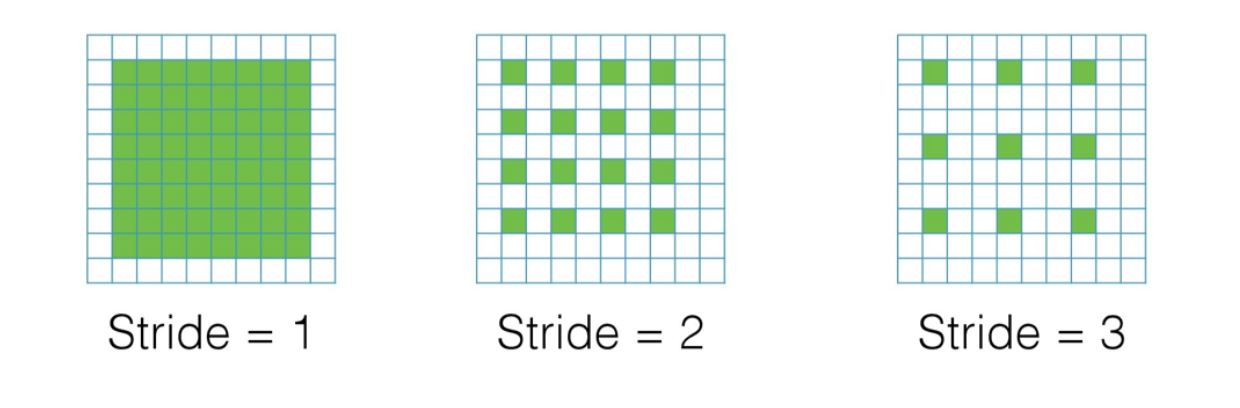
\includegraphics[width=.8\linewidth]{stride.png}
	\end{center}
\end{frame}


\begin{frame}{Свёртки с пропусками (strides)}
\begin{center}
	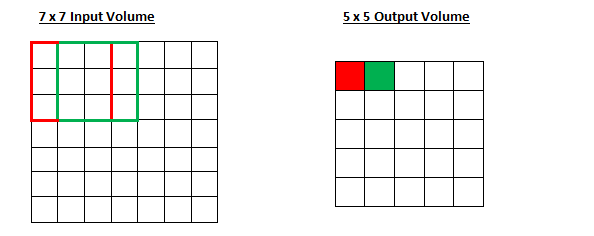
\includegraphics[width=.6\linewidth]{Stride1.png}
\end{center}
\vfill
\begin{center}
	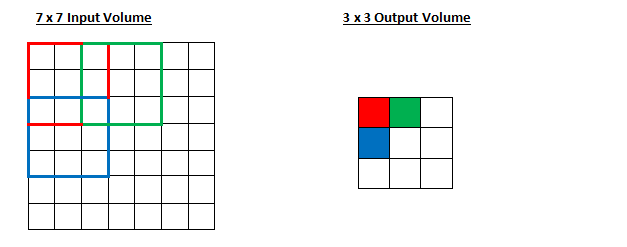
\includegraphics[width=.6\linewidth]{Stride2.png}
\end{center}
\end{frame}


\begin{frame}{Пулинг слой (Pooling)}
	\begin{itemize}
		\item  Внутри какого-то окна ишем максимум или среднее, размер изображения существенно сокращается, а поле восприятия растёт
	\end{itemize}
	
	\begin{center}
		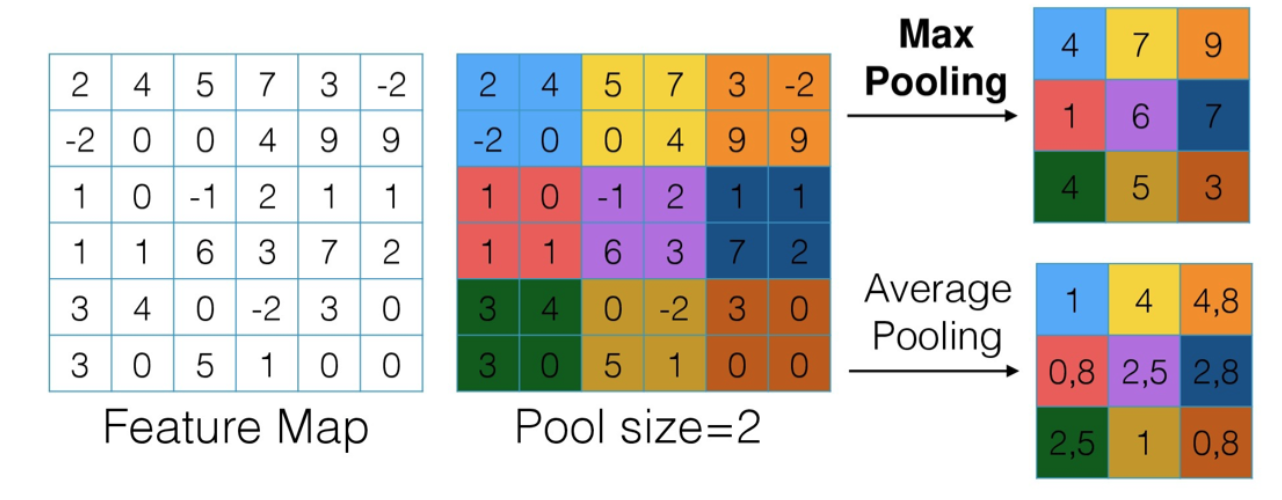
\includegraphics[width=.7\linewidth]{pooling.png}
	\end{center}
\end{frame}


\begin{frame}{Как считать градиент для пулинга?}
	\begin{wideitemize}
		\item строго говоря: максимум не дифференцируемая функция
		\item Градиент 0 по немаксимальным входам, потому что при их изменении не меняется выход (максимум)
		\item Для максимального входа градиент 1.		
	\end{wideitemize}			
	\begin{center}
		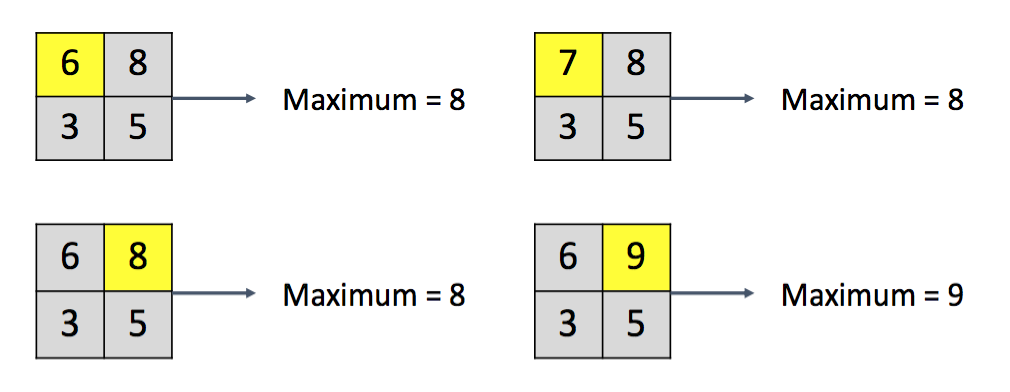
\includegraphics[width=.7\linewidth]{pooling_grad.png}
	\end{center}
\end{frame}



\begin{frame}{Зачем это всё?}
	\begin{wideitemize}
	\item  Важно следить за тем, чтобы последние свёрточные слои имели размер поля восприятия, сравнимый со всей картинкой
	
	\item Нужно понимать, что для более сложных арихитектур (батч-норм, скип-конекшн) поле обзора вычисляется сложнее, у пикселей есть больше маршрутов в рамках нейросетки
	\end{wideitemize}
\end{frame}



\begin{transitionframe}
	\begin{center}
		\Huge  Простейшие свёрточные сети
	\end{center}
\centering 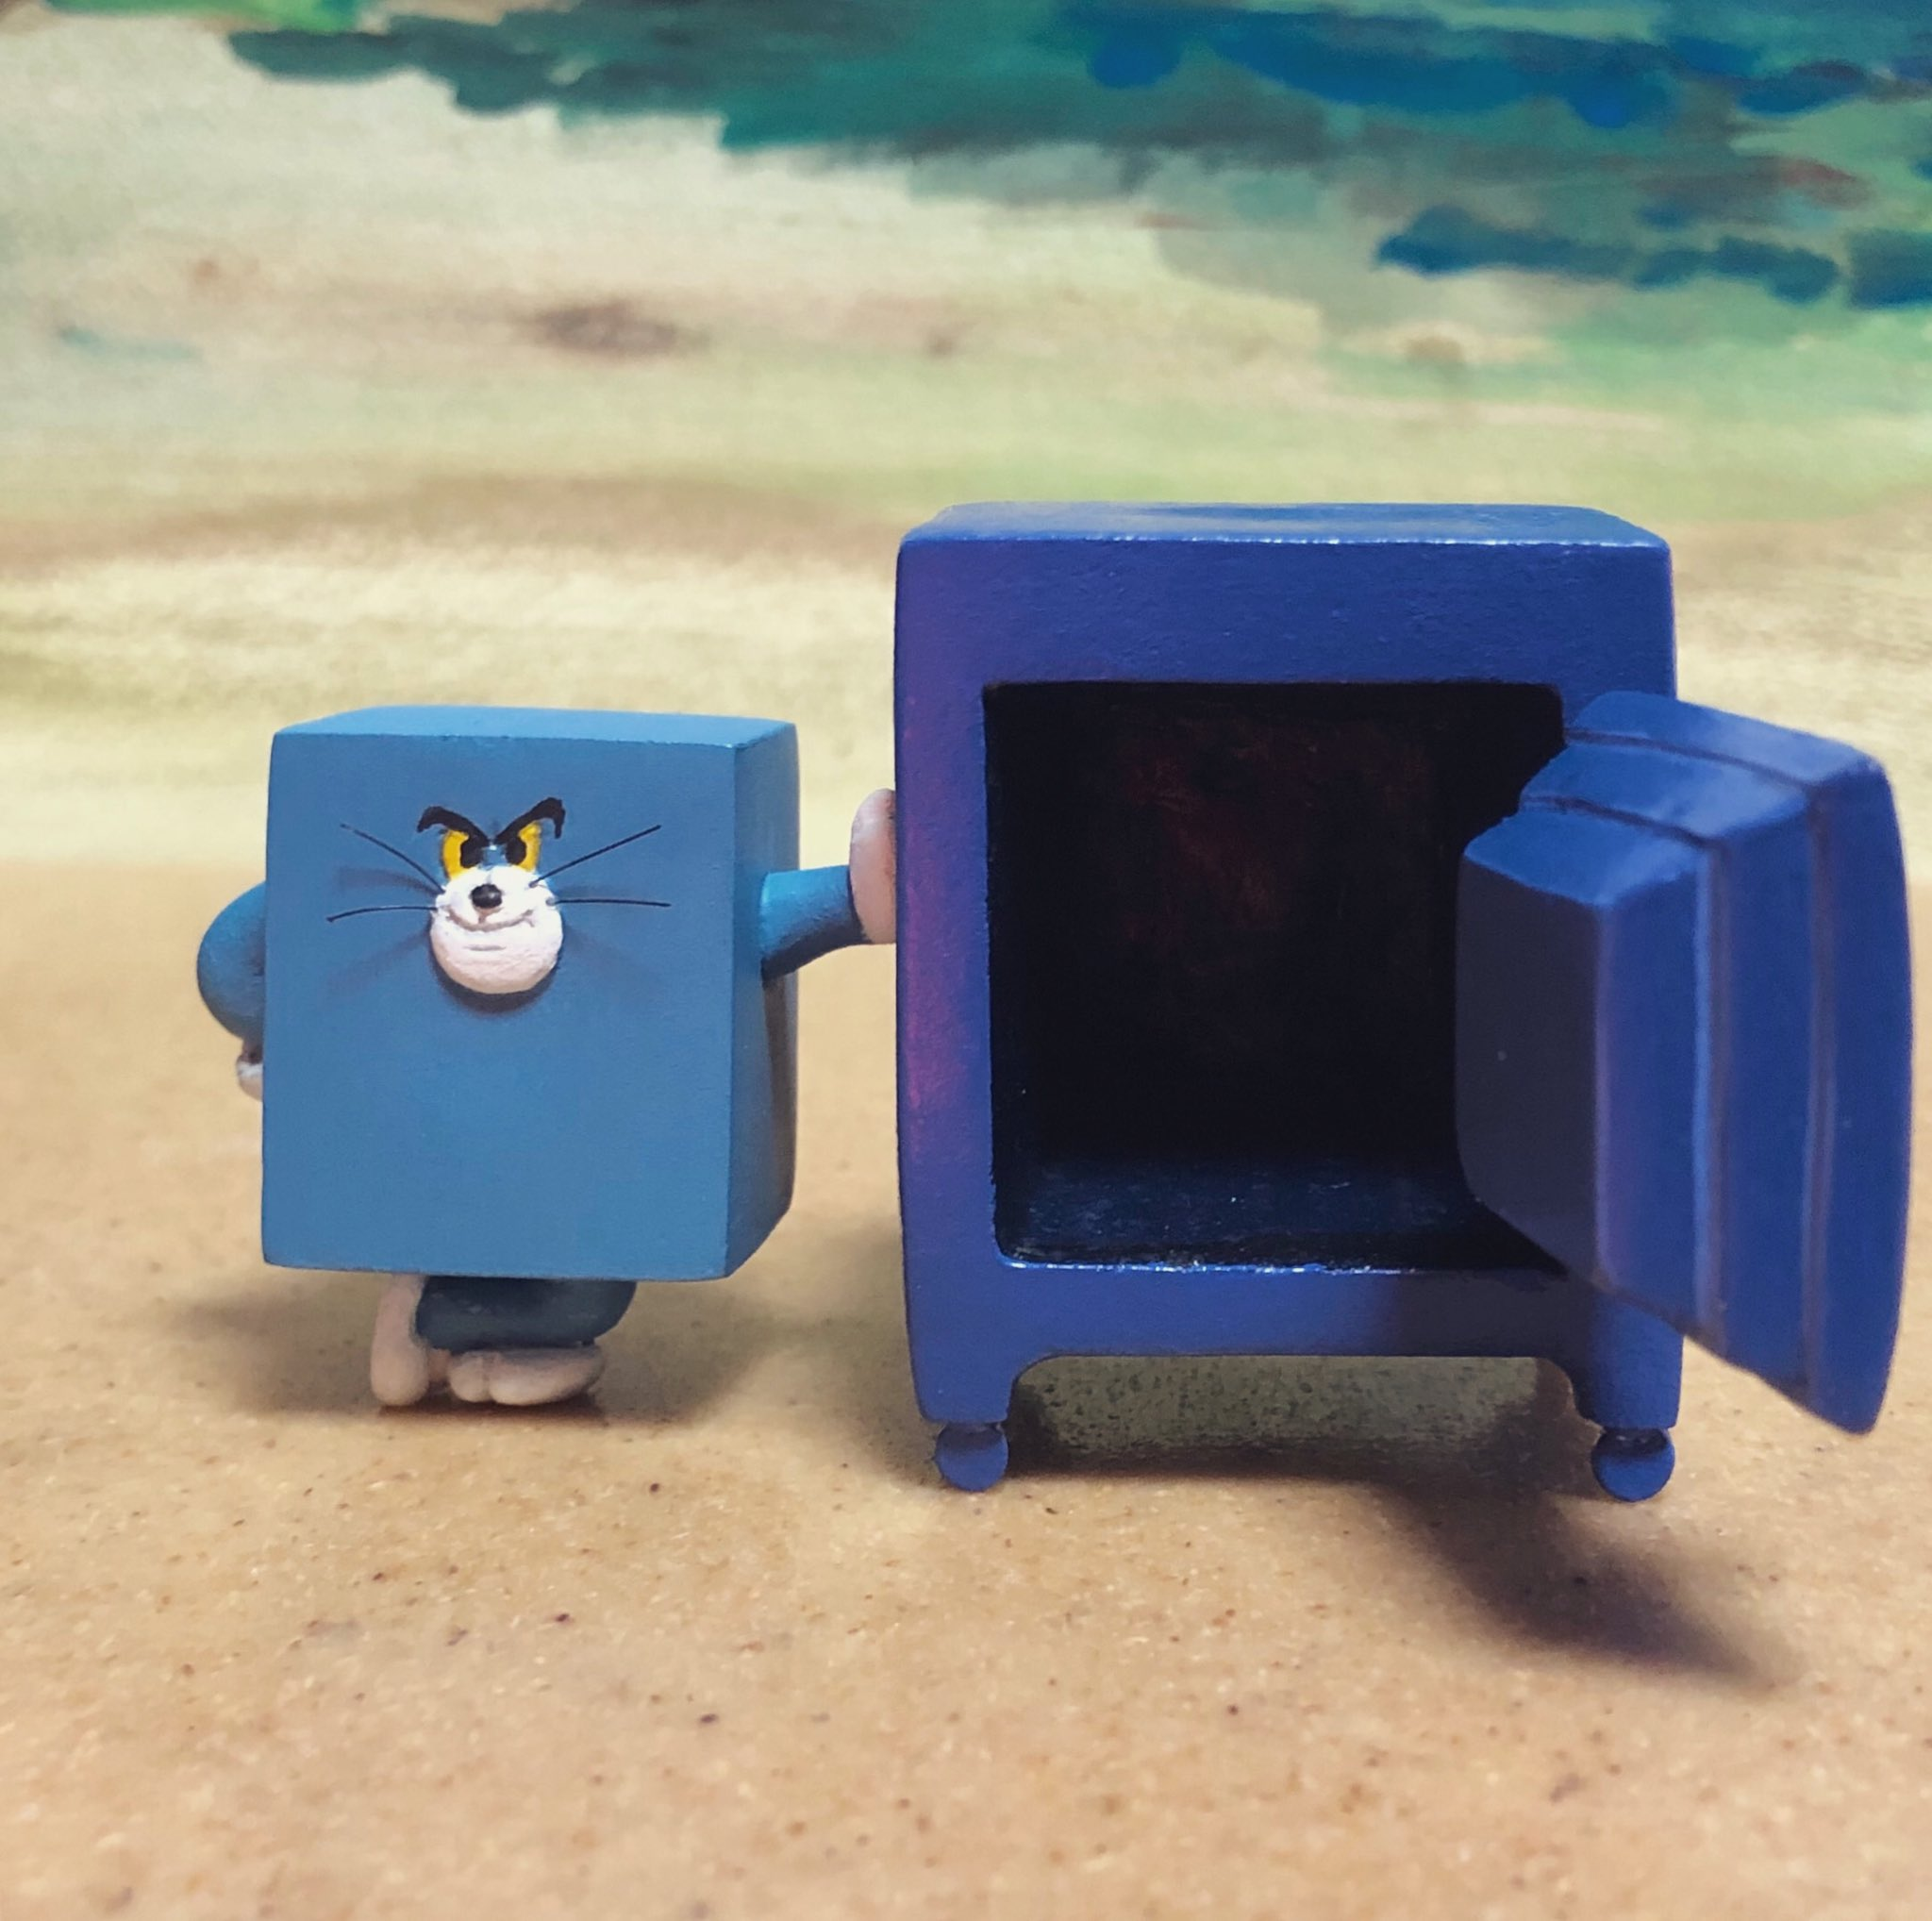
\includegraphics[scale = 0.05]{corner_tom.jpg}
\end{transitionframe}


\begin{frame}{Типичная архитектура}
\begin{center}
	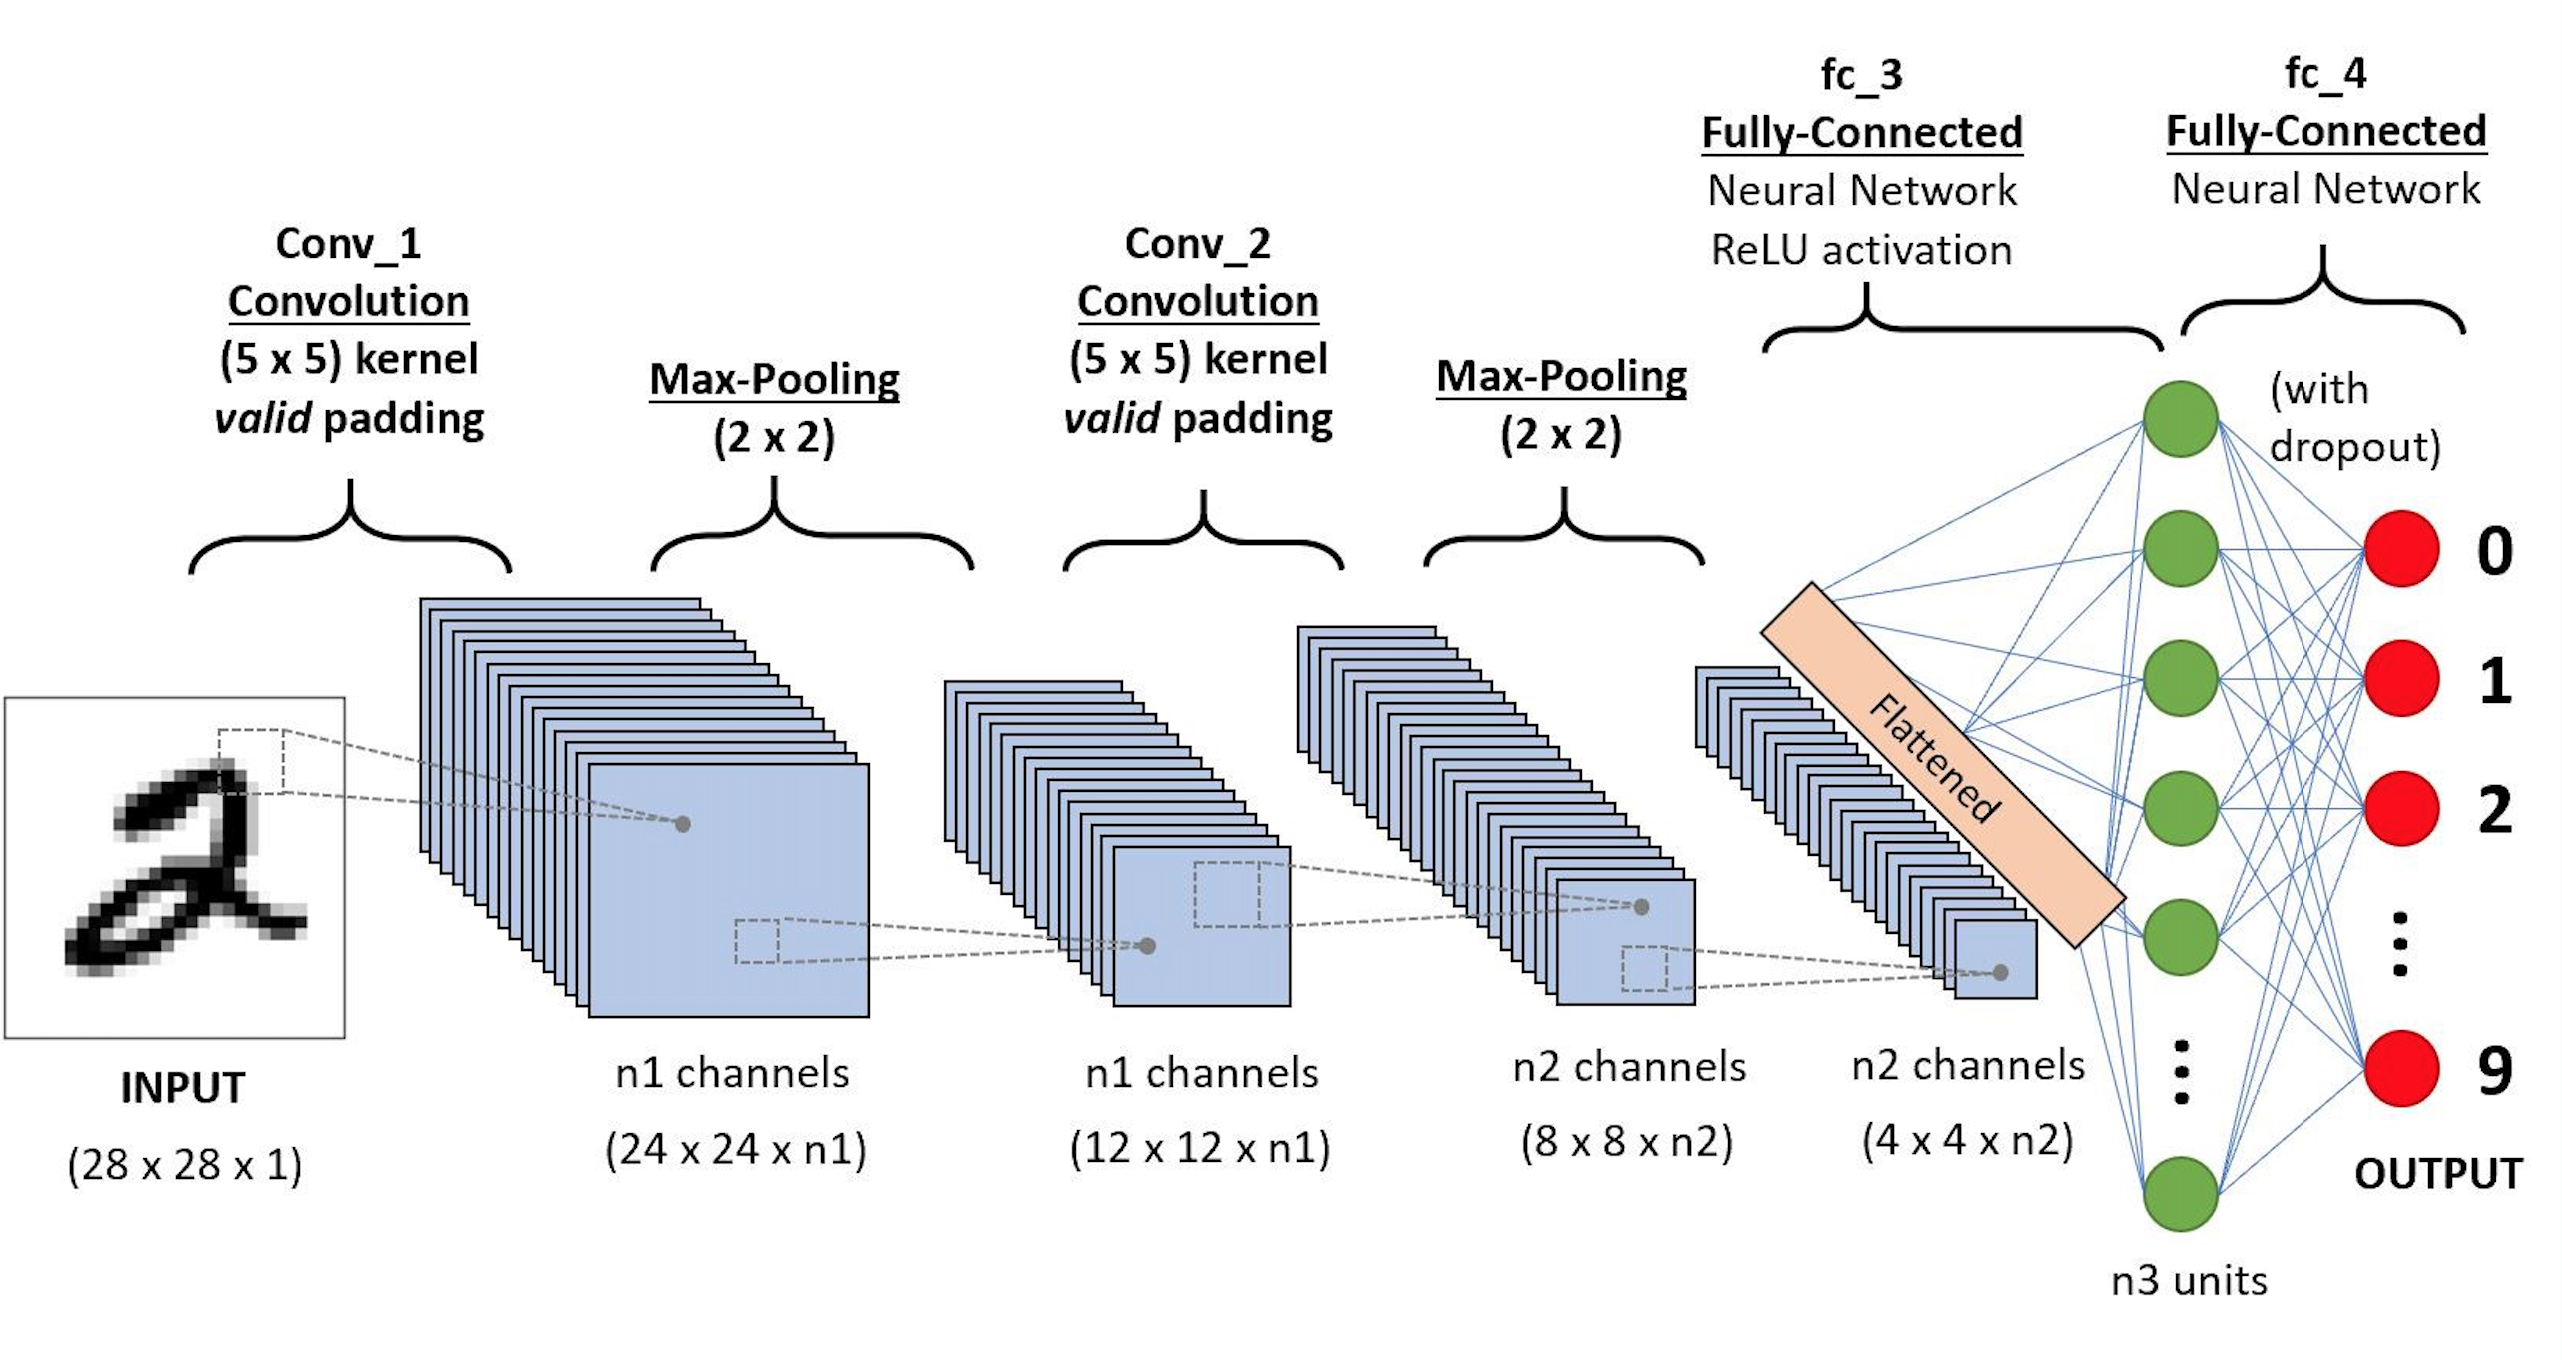
\includegraphics[width=.8\linewidth]{nn_tp.png}
\end{center}

\vfill
\scriptsize
{\color{blue} \url{https://towardsdatascience.com/a-comprehensive-guide-to-convolutional-neural-networks-the-eli5-way-3bd2b1164a53}}
\end{frame}


\begin{frame}{Типичная архитектура}
\begin{wideitemize}
	\item   Последовательное применение комбинаций вида: свёрточный слой $\Rightarrow$ нелинейность $\Rightarrow$ pooling
	\item  Выпрямление (flattening) выхода очередного слоя
	\item  Серия полносвязных слоёв
\end{wideitemize}
\end{frame}


\begin{frame}{Типичная архитектура}
	\begin{center}
		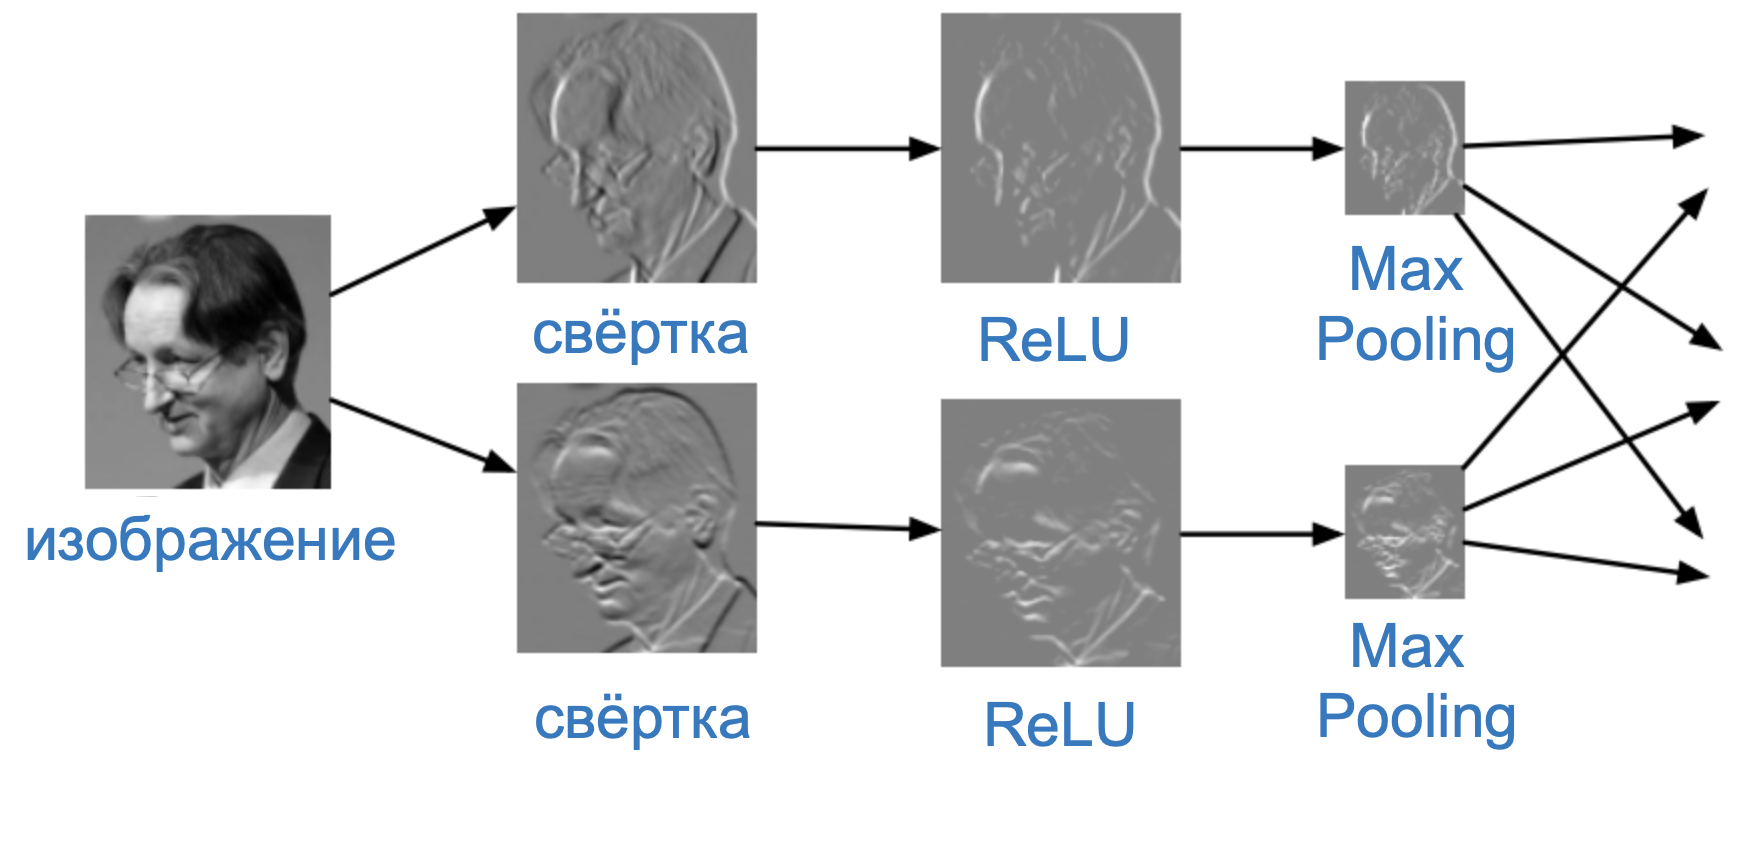
\includegraphics[width=.9\linewidth]{conv_man.png}
	\end{center}
\end{frame}


\begin{frame}{LeNet (1998)}
	\begin{center}
		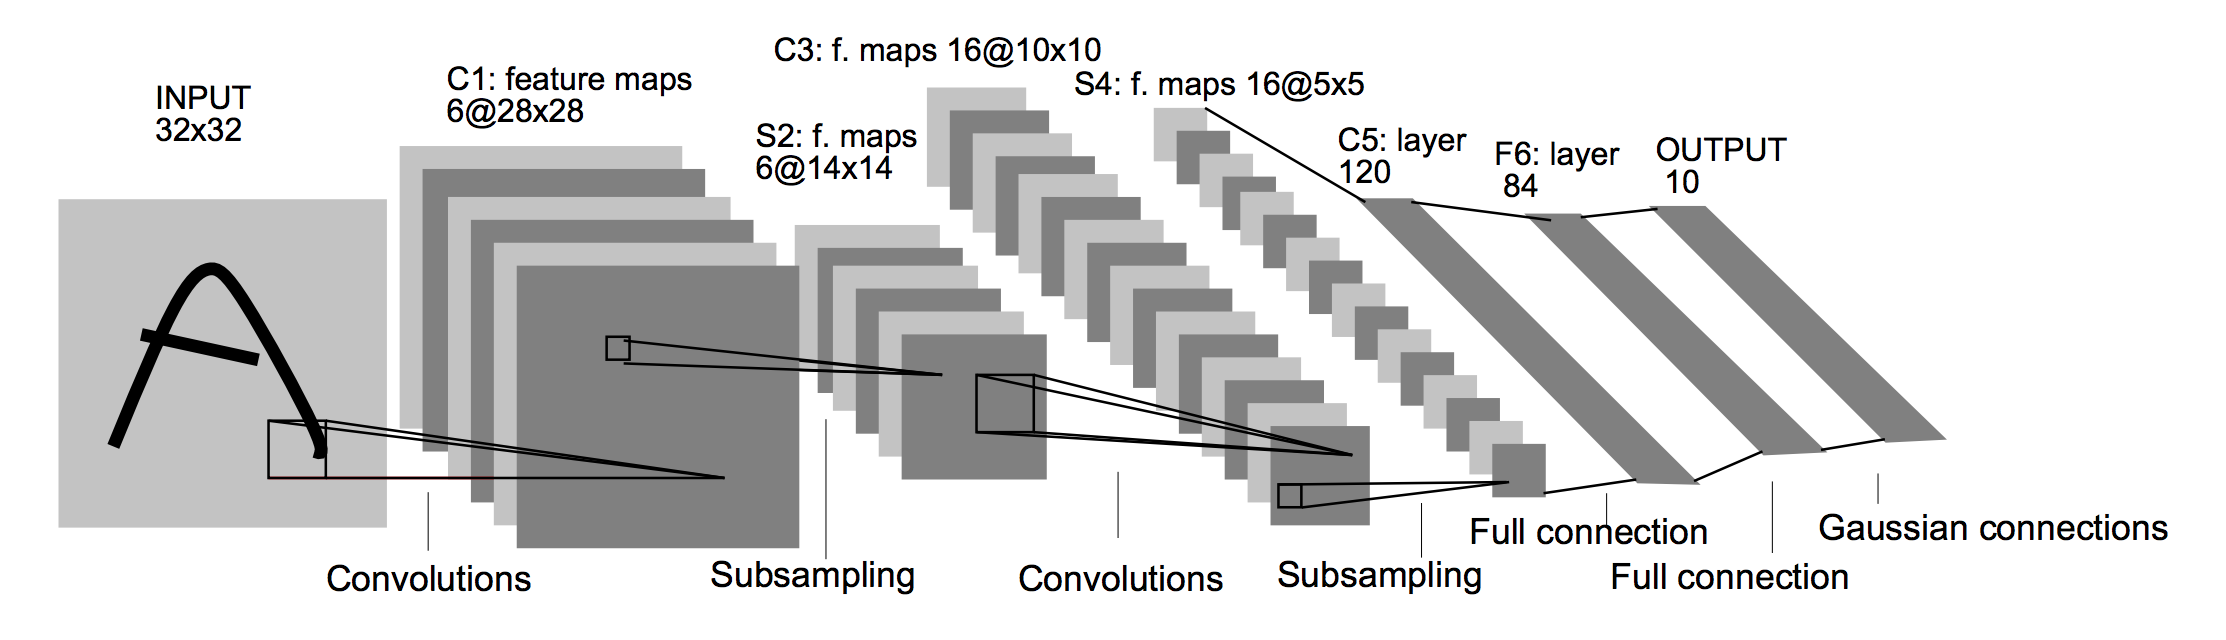
\includegraphics[width=.99\linewidth]{lenet.png}
	\end{center}
	\vfill
	\scriptsize
	{\color{blue} \url{http://yann.lecun.com/exdb/publis/pdf/lecun-98.pdf}}
\end{frame}


\begin{frame}{AlexNet (2012)}
	\begin{center}
		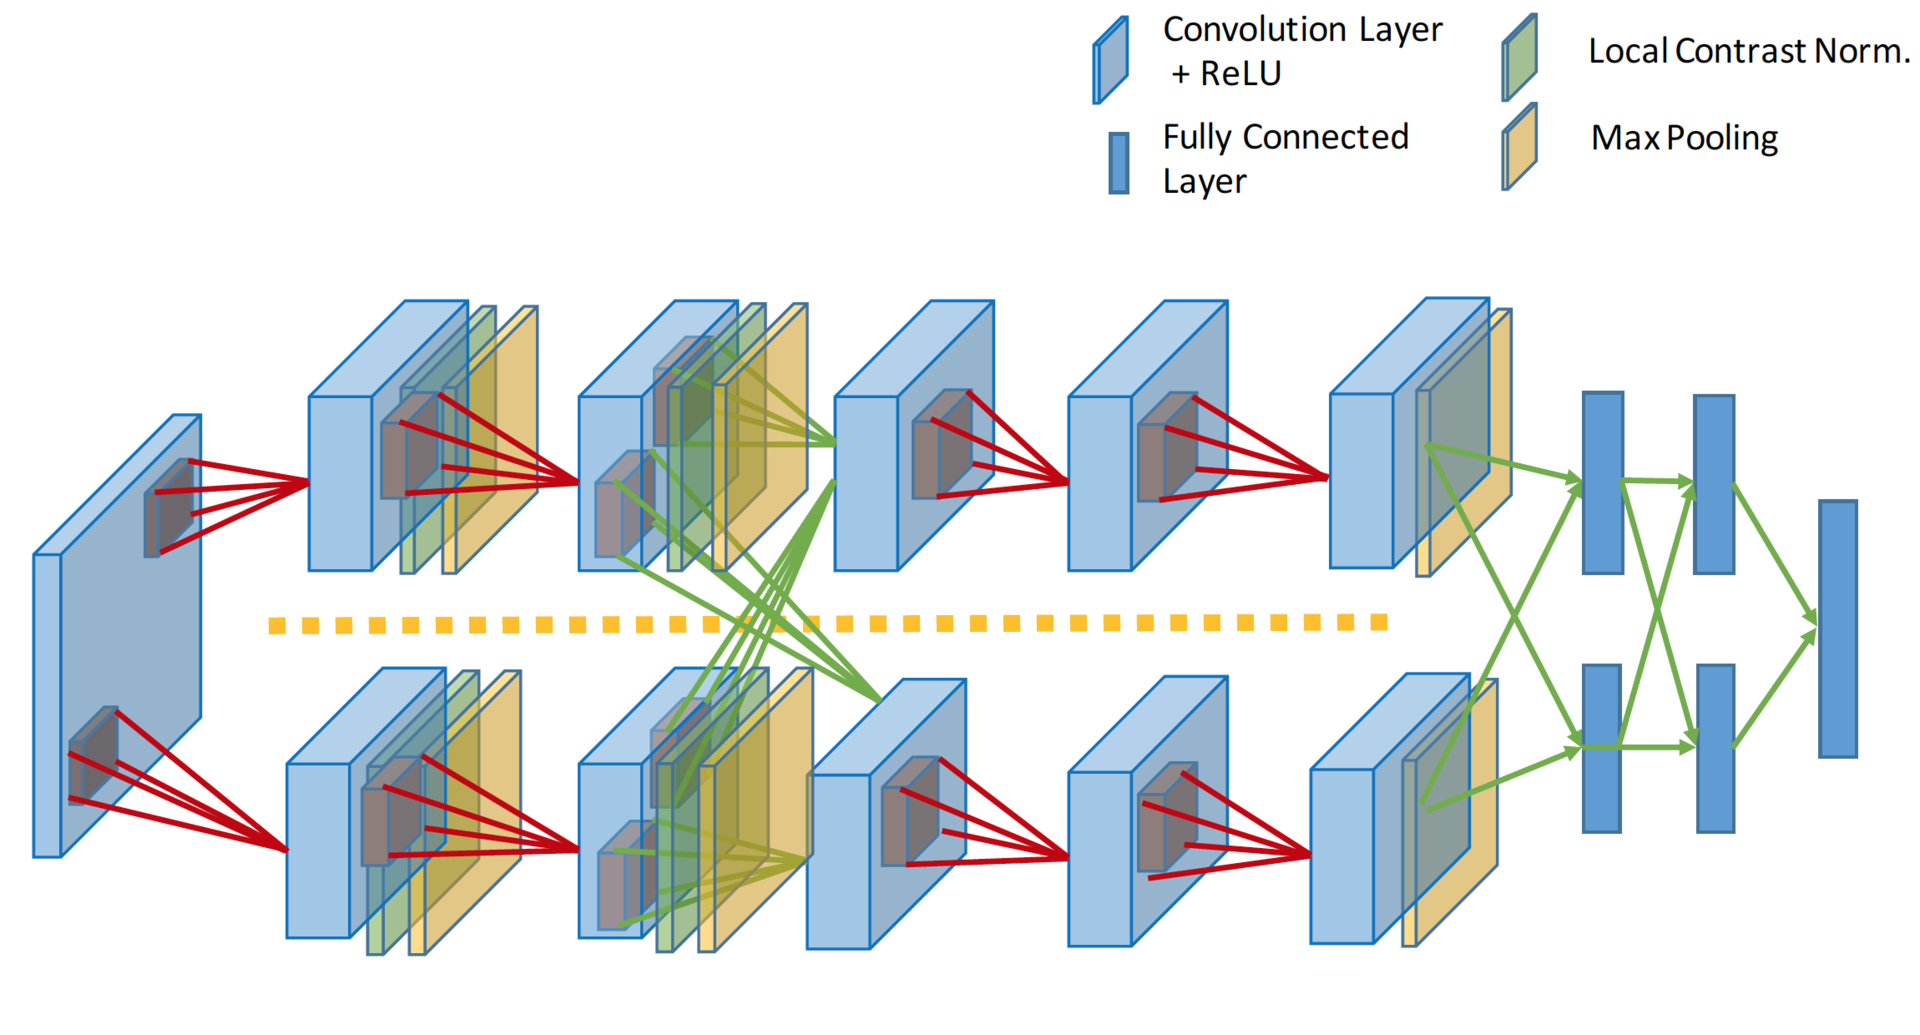
\includegraphics[width=.8\linewidth]{alexnet.png}
	\end{center}
	\vfill
	\scriptsize
	{\color{blue} \url{http://papers.nips.cc/paper/4824-imagenet-classification-with-deep-convolutional-neural-networks.pdf}}
\end{frame}


\begin{transitionframe}
	\begin{center}
		\Huge  Что выучивают нейросети
	\end{center}
\centering 
\includegraphics[scale = 0.5]{read_tom.jpg}
\end{transitionframe}


\begin{frame}{Что выучивают нейросети}
\begin{center}
	\includegraphics[width=0.73\paperwidth]{network_1.png}
\end{center}
\end{frame}


\begin{frame}{Что выучивают нейросети}
\begin{wideitemize}
	\item Первые слои выучивают какие-то низкоуровневые вещи по типу углов/краёв/линий
	\item Последние слои реагируют уже на целые части изображений
	\item  Нейросеть учит иерархические шаблоны
\end{wideitemize}
\end{frame}


\begin{frame}{Что выучивают нейросети}
\begin{center}
	\includegraphics[width=0.3\paperwidth]{layer1.png}
\end{center}
\vfill
\footnotesize
{\color{blue} \url{https://arxiv.org/pdf/1311.2901.pdf}}
\end{frame}


\begin{frame}{Что выучивают нейросети}
\begin{center}
	\includegraphics[width=0.73\paperwidth]{layer_3.png}
\end{center}
\vfill
\footnotesize
{\color{blue} \url{https://arxiv.org/pdf/1311.2901.pdf}}
\end{frame}


\begin{frame}{Что выучивают нейросети}
\begin{center}
	\includegraphics[width=0.73\paperwidth]{layer_2.png}
\end{center}
\vfill
\footnotesize
{\color{blue} \url{https://arxiv.org/pdf/1311.2901.pdf}}
\end{frame}


\begin{frame}{Что выучивают нейросети}
\begin{center}
	\includegraphics[width=0.73\paperwidth]{layer_45.png}
\end{center}
\vfill
\footnotesize
{\color{blue} \url{https://arxiv.org/pdf/1311.2901.pdf}}
\end{frame}


\begin{frame}{Демо: визуализация обученной сети для MNIST}
\begin{center}
	\includegraphics[width=0.7\paperwidth]{mnist_demo.png}
\end{center}
\vfill
\footnotesize
{\color{blue} \url{http://scs.ryerson.ca/~aharley/vis/conv/flat.html}}
\end{frame}


\begin{frame}{Представления с последних слоёв}
\begin{wideitemize}
	\item  Выходы с последних слоёв свёрточных нейросетей являются хорошими признаковыми описаниями изображений
	\item Такие векторные представления называют \alert{эмбеддингами (embeddings)}
	\item У эмбеддингов нет чёткой интерпретации, цифры в них говорят о наличии каких-то паттернов, на которые настроилась нейросетка
	\item Эмбеддинги картинок оказываются полезными во многих задачах 
\end{wideitemize}
\end{frame}


\begin{transitionframe}
	\begin{center}
		\Huge  Снятся ли нейросетям электрические овцы?
	\end{center}
	\centering \includegraphics[scale = 0.3]{shon.png}
\end{transitionframe}


\begin{frame}{Найдите на картинке овцу}
\begin{center}
	\includegraphics[width=0.65\linewidth]{sheep1.png}
\end{center}
\vfill
\footnotesize
{\color{blue} \url{https://www.aiweirdness.com/do-neural-nets-dream-of-electric-18-03-02/}}
\end{frame}


\begin{frame}{Найдите на картинке овцу}
\begin{center}
	\includegraphics[width=0.65\linewidth]{sheep2.png}
\end{center}
\vfill
\footnotesize
{\color{blue} \url{https://www.aiweirdness.com/do-neural-nets-dream-of-electric-18-03-02/}}
\end{frame}


\begin{frame}{Найдите на картинке цветы}
\begin{center}
	\includegraphics[width=0.65\linewidth]{sheep3.png}
\end{center}
\vfill
\footnotesize
{\color{blue} \url{https://www.aiweirdness.com/do-neural-nets-dream-of-electric-18-03-02/}}
\end{frame}


\begin{frame}{Найдите на картинке птиц}
\begin{center}
	\includegraphics[width=0.65\linewidth]{sheep4.png}
\end{center}
\vfill
\footnotesize
{\color{blue} \url{https://www.aiweirdness.com/do-neural-nets-dream-of-electric-18-03-02/}}
\end{frame}



\begin{transitionframe}
	\begin{center}
		\Huge  Собираем свою собственную CNN
	\end{center}
\end{transitionframe}


\end{document}
